\chapter{Results}
\label{chap:results}

The basis for setting a pulse height discriminator to differentiate between neutron and gammas can be attributed to the secondary electrons and the difference in energy mechanisms as presented later.
However, the application to physical detectors has yet to be concretely formulated.
This section will serve to remedy that and present a pulse height discrimination scheme capable of discrimination between neutrons and gammas.

It is currently understood that the light output per path length of the film (which is directly proportional to the pulses collected on the PMT) is related to the stopping power of the radiation in the film material.
For a given material the stopping power of the film will be constant, and therefore the light output of the film can be found by integrating the light output per path length over the total length of the film.
It is then possible to conclude that the light output of a film is proportional to the energy deposited in the film.

Preferential energy deposition by neutrons relative to gammas will enhance the discrimination by creating larger neutron light pulses than the gamma pulses, allowing for fewer neutron pulses to be classified as gamma pulses because they are below the MLLD.
Thus, neutron-gamma discrimination can be enhanced by optimizing the energy deposition in the film. 

\section{Energy Deposition}
%%%%%%%%%%%%%%%%%%%%%%%%%%%%%%%%%%%%%%%%%%%%%%%%%%%%%%%%%%%%%%%%%%%%%%%%%%%
%                                                                         %
%                     ENERGY DEPOSITION SIMULATIONS                       %
%                                                                         %
%%%%%%%%%%%%%%%%%%%%%%%%%%%%%%%%%%%%%%%%%%%%%%%%%%%%%%%%%%%%%%%%%%%%%%%%%%%

The average energy deposited by a neutron and gamma reaction was investigated for different film thickness to determine if an optimal thickness exits in a geometry similar to \autoref{fig:EDepSimGeo}.
\autoref{fig:SimEDep} shows that the energy deposition of the gamma quickly falls off as the films get thinner, while it isn't until the neutron films become on the order of the range of the triton that the energy deposition is impacted.
\begin{figure}
  \centering
  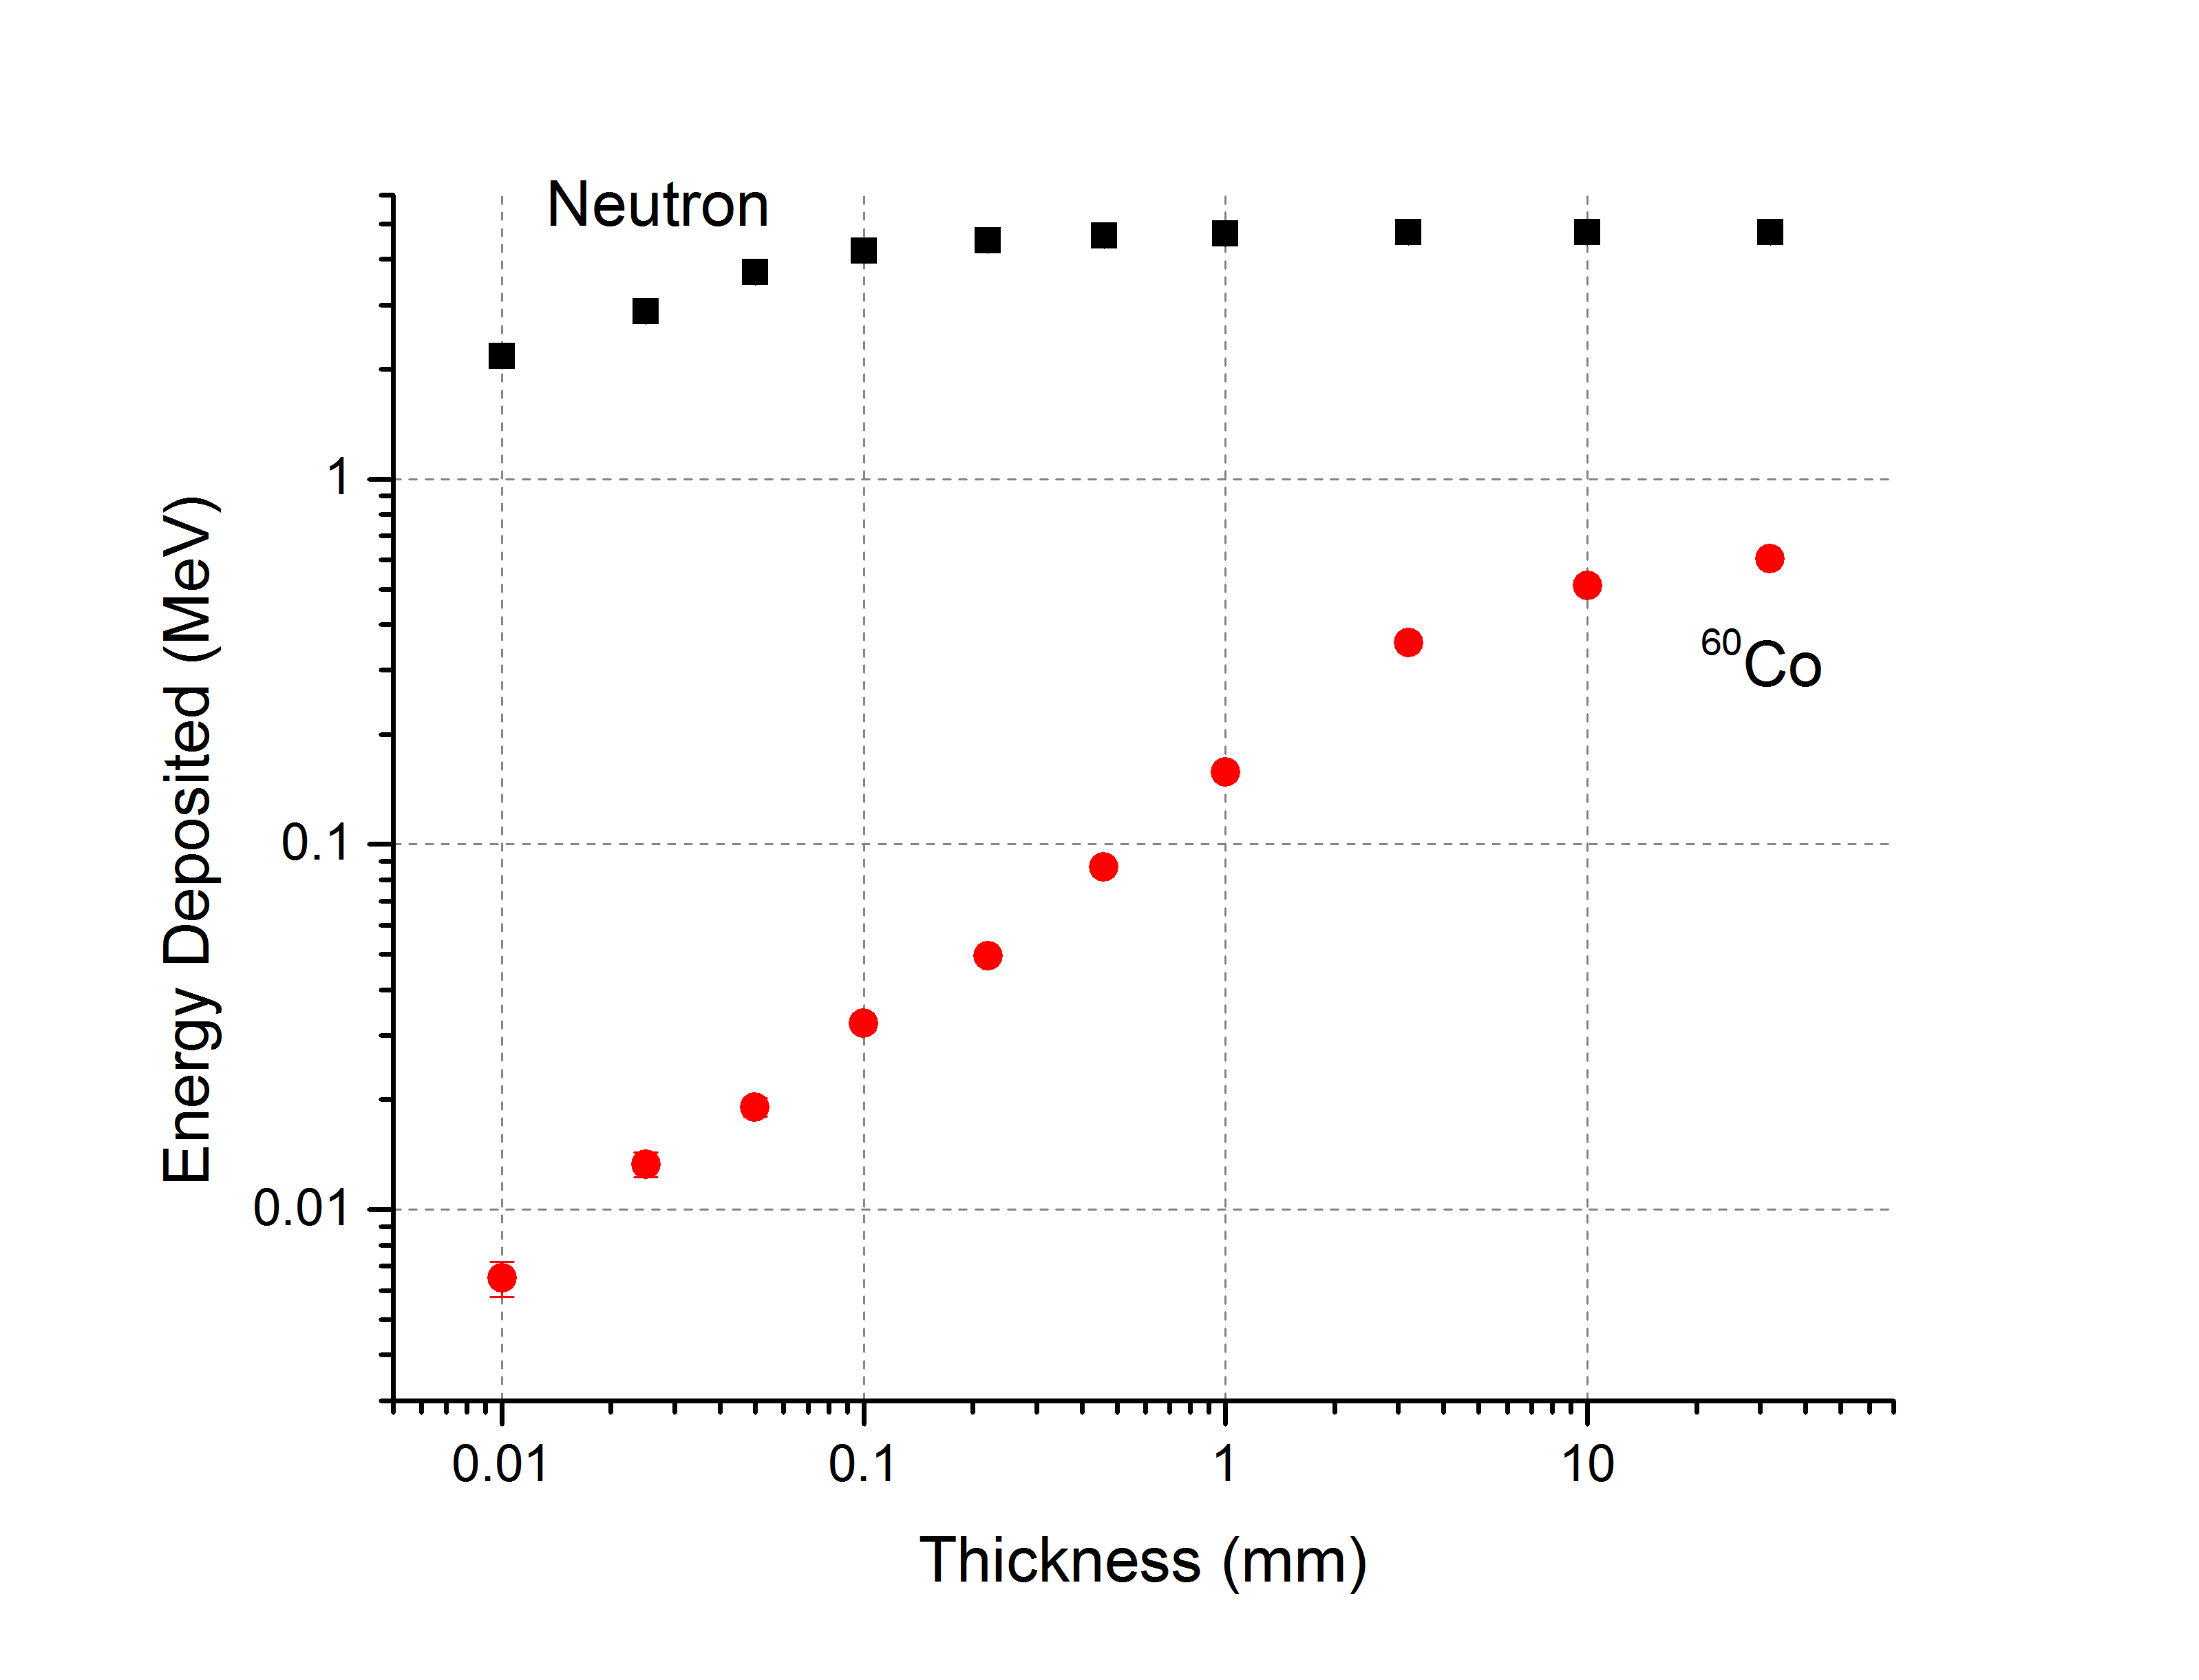
\includegraphics[width=\textwidth]{SimulatedEnergyDeposition}
  \caption[Simulated Energy Deposition and Film Thickness]{Simulated energy deposition and film thickness. As the films get thinner it is very unlikely for gamma events (and their secondary electrons) to deposition all of their energy, while above \SI{50}{\um} there is very little impact on the energy deposited by neutrons.\EnergyDepSimGeo}
  \label{fig:SimEDep}
\end{figure}

Interactions that occur near the edge of the film may have a large impact in the energy absorbed in the film for very thin films where a large fraction of the volume is within a mean free path of the surface of the detector material.
For example, for a \SI{25}{\um} film the range of the triton exceeds the thickness of the film.
The energy loss of interactions occurring near the edge of the film was investigated by simulating the energy loss for a large planar detector where the beam spot is \SI{3}{\mm} and the area of the detector face is \SI{10}{\cm}. 
The geometry for this simulation shown in \autoref{fig:EDepSimGeo}, with the interaction position defined to be distance to the first interaction of the beam in the material along the direction of the beam.
\autoref{fig:EDepPosSim} examines the impact of where the interaction took place in the film on the energy deposition.
It is observed that for neutrons events that take place within the center of the films tend to deposit a large majority of their energy in the film, while events that occur on the edge of the film have partial energy depositions in accordance with the ranges of the charged particles.
The Compton edge is observed at \SI{1}{\MeV} in the simulated photon energy deposition for the \SI{1}{\cm} film, as expected.
A secondary effect in having a backing material is also observed for photons in which there is a heightened energy deposition for interactions that occur in the film but near the boundary and electrons are back scattered into the detector material.
\begin{figure*}[ht]
	\centering
	\begin{subfigure}[b]{0.45\textwidth}
    		\includegraphics[width=\textwidth]{{posEDepCo600.025}.png}
		\caption{ \SI{25}{\um} Gamma (\iso[60]{Co})}
	\end{subfigure}%
	~
	\begin{subfigure}[b]{0.45\textwidth}
    		\includegraphics[width=\textwidth]{{posEDepCo6010.0}.png}
		  \caption{ \SI{1}{\cm} Gamma (\iso[60]{Co})}
	\end{subfigure}%
	
  \begin{subfigure}[b]{0.45\textwidth}
    		\includegraphics[width=\textwidth]{{posEDepneutron0.025}.png}
		\caption{ \SI{25}{\um} Neutron}
	\end{subfigure}%
	~
	\begin{subfigure}[b]{0.45\textwidth}
    		\includegraphics[width=\textwidth]{{posEDepneutron10.0}.png}
		  \caption{ \SI{1}{\cm} Neutron}
	\end{subfigure}%
	\caption[Simulated Energy Deposition and Position]{Simulated average energy depositions and the position of the first interactions. The beam is considered to be incident on position 0, and thus interactions that occur on the front of the film have a much higher probability depositing all of their energy. Events that occur on the edge of the film much less likely to deposit all of their available energy.}
	\label{fig:EDepPosSim}
\end{figure*}

\autoref{fig:simKinE} illustrates the simulated kinetic energy of secondary electrons from Compton scattering and from alpha and triton interactions.
It is observed that kinetic energy of the secondary electrons from the neutron reaction products have predominately energies in the kilo-volt range, while the Compton scattering electrons have energies in hundreds of kilo-volts range. 
However, it should be noted that there is only one secondary electron from a Compton scattering and multiple secondary electrons from the reaction products.
The kinetic energy distribution is broken down by the two reaction products in \autoref{fig:SecElecKinEDist}, while relative number of secondary electrons is shown in \autoref{fig:ReacProdDist}.
It is apparent that the triton contributes more secondary electrons than heavier alpha, while they have similar energies of the secondary electrons.
\begin{figure}[ht]
    \centering
    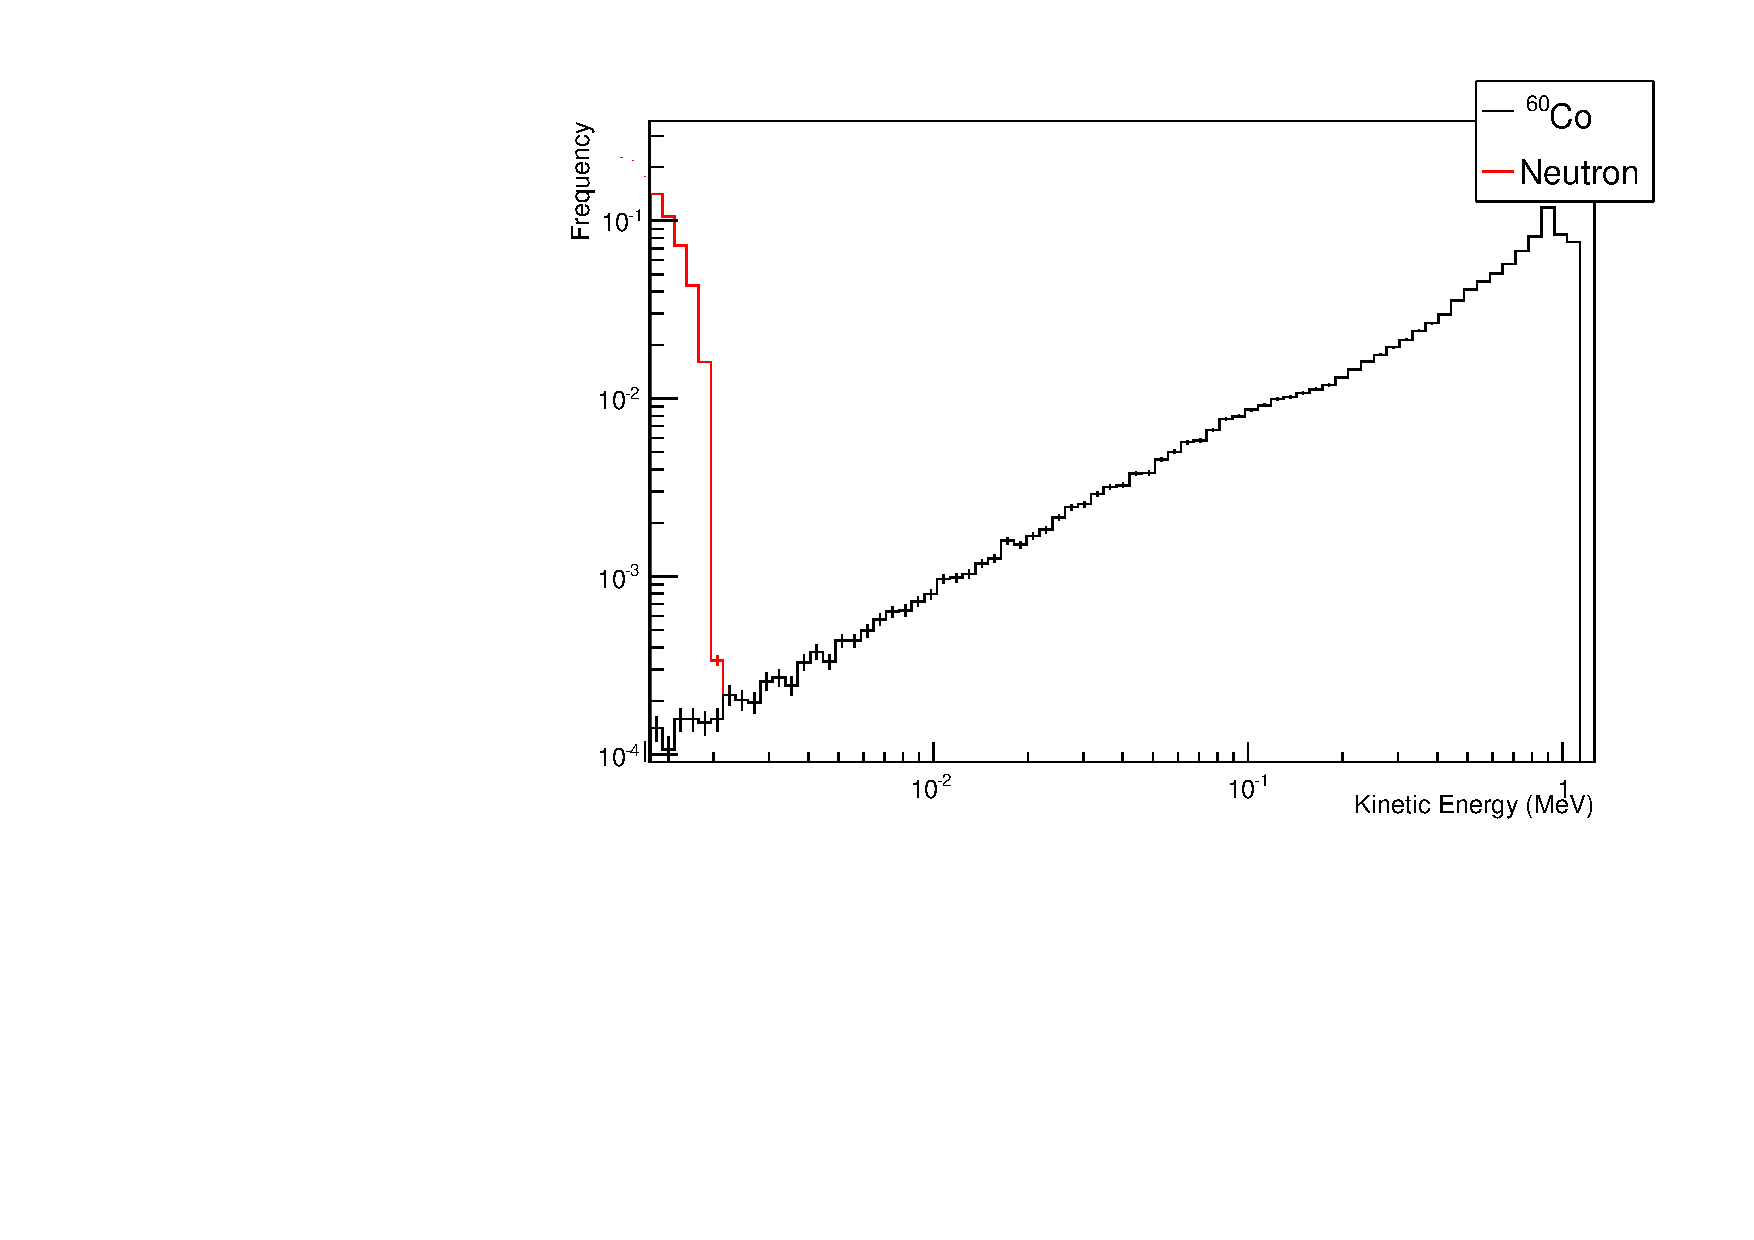
\includegraphics[width=\textwidth]{NGSecElecKinEDist}
    \caption[Kinetic Energy of Primary Secondary Electron from Compton Scattering and Neutron Reaction Prodcuts]{The kinetic energy of the first secondary electron from compton scattering with \iso[60]{Co} and from \iso[6]{Li} reaction products. The energy distrubtion of all of the electrons produced in the interactions is shown in \autoref{fig:ERangeAndDist}.\EnergyDepSimGeo}
    \label{fig:simKinE}
\end{figure}
\begin{figure}
 	\centering
  	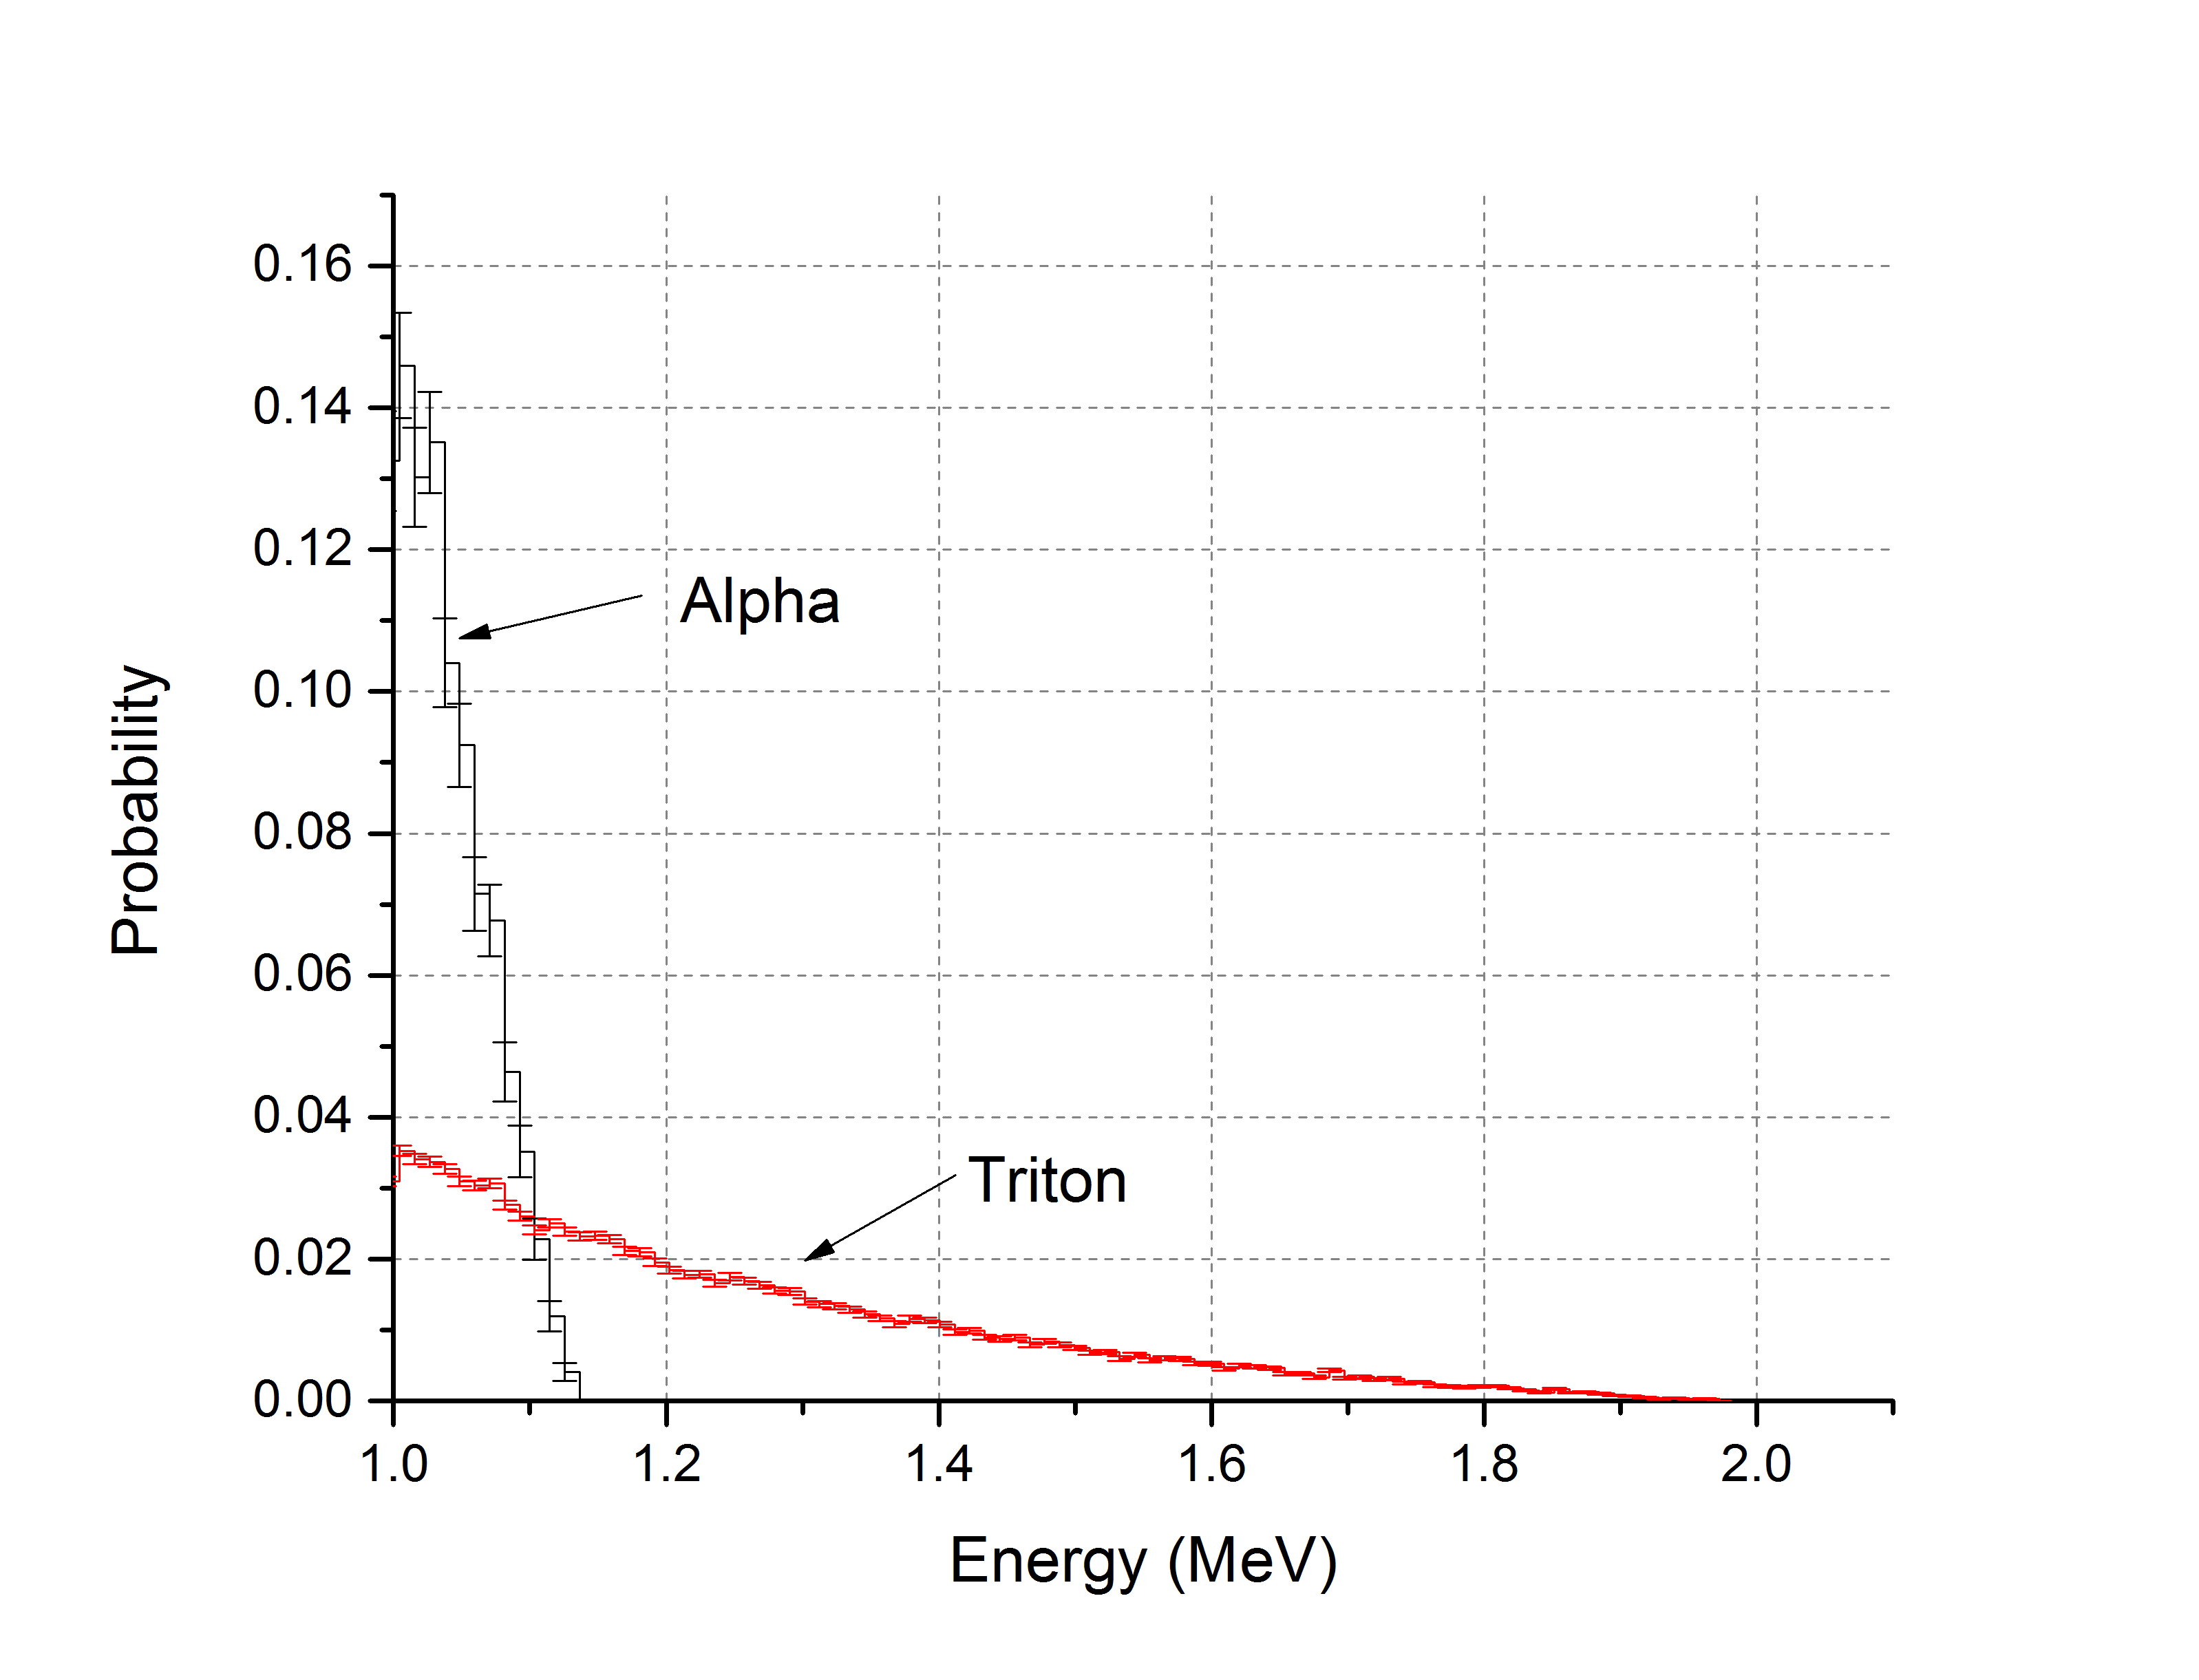
\includegraphics[width=\textwidth]{AlphaTritonSecElecKinEDist}
	\caption[Kinetic Energy Distribution of Primary Secondary Electrons from the Neutron Reaction Products]{Kinetic energy distribution of the first secondary of the neutron reaction products (alpha and tritron) from a \iso[6]{Li} interaction.  Most of the electrons have kinetic energies in the \SI{1}{\keV} range. \EnergyDepSimGeo}
	\label{fig:SecElecKinEDist}
\end{figure}
\begin{figure}
 	\centering
  	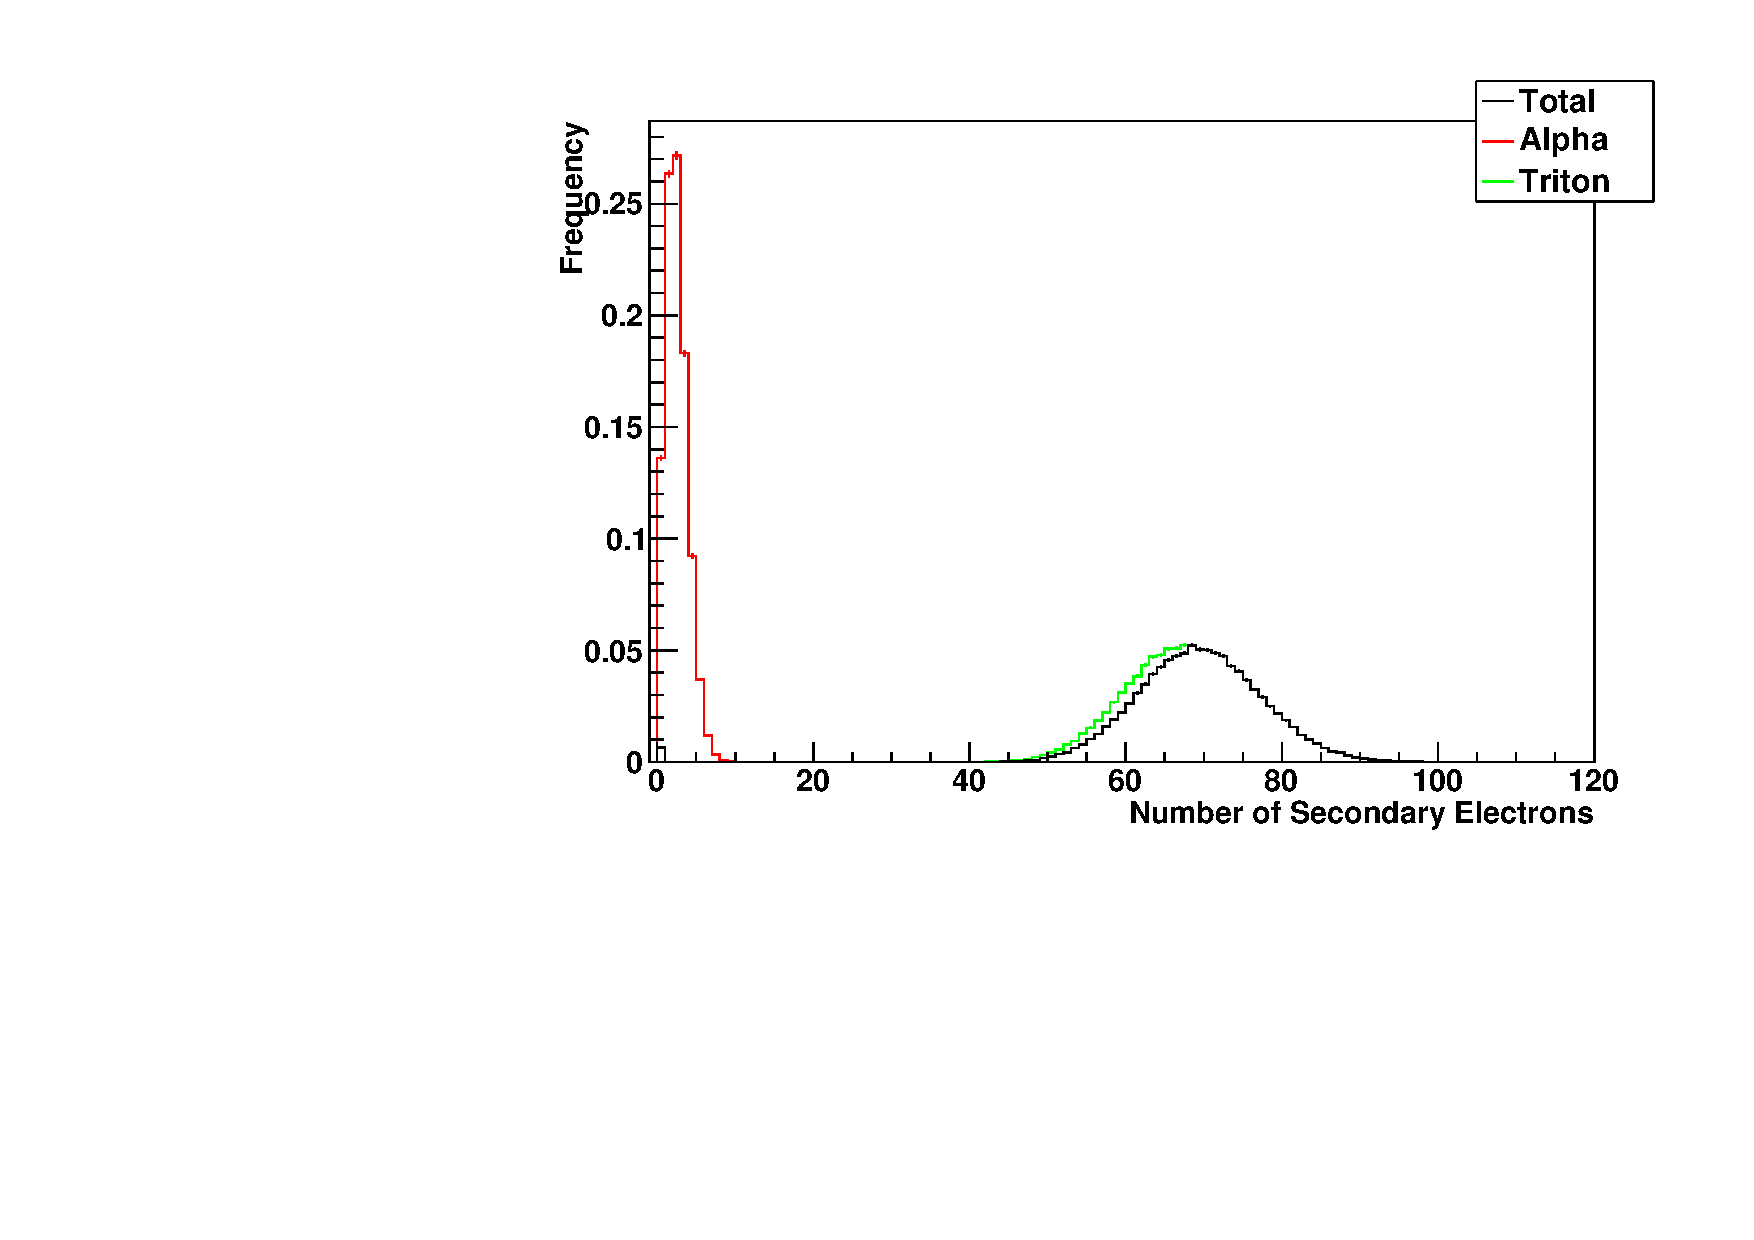
\includegraphics[width=\textwidth]{NeutronNumSecElec}
	\caption[Distribution of the Number of Secondary Electrons Produced Per Neutron Interaction]{Distribution of the Number of Secondary Electrons Produced Per Neutron Interaction. The alpha particle produces almost a factor of 16 less photons than the triton. \EnergyDepSimGeo}
	\autoref{fig:ReacProdDist}
\end{figure}

The average energy deposited was computed for each thickness and normalized by the incident energy for gammas by the Q-value of the reaction for neutrons, and is presented in \autoref{tab:FractionEDep}.
For thickness greater than \SI{150}{\um} there is little benefit in increasing the thickness of the film in terms of energy deposition by neutrons, since over 90\% of the energy is being deposited in the film.
\begin{table}
    \caption[Fractional Energy Deposition per Interaction for Various Thickness]{Fraction of total energy deposited per interaction of a neutron and the photons from \iso[60]{Co} in films of various thickness. The total energy deposited in a neutron event is \SI{4.78}{\MeV}, while the maximum energy deposited from a \iso[60]{Co} is \SI{1.33}{\MeV}.\EnergyDepSimGeo}
	\centering
	\begin{tabular}{c | c c}
	Thickness & Gamma Fraction & Neutron Fraction \\
	\hline
	\hline
	\SI{15}{\um} & 0.010 & 0.531 \\
	\SI{25}{\um} & 0.013 & 0.634 \\
	\SI{50}{\um} & 0.017 & 0.782 \\
	\SI{150}{\um} & 0.032 & 0.927 \\
	\SI{300}{\um} & 0.052 & 0.964 \\
	\SI{600}{\um} & 0.087 & 0.982 \\
	\SI{1}{\mm} & 0.130 & 0.989 \\
	\SI{1}{\cm} & 0.425 & 0.998 \\
	\end{tabular}
  \label{tab:FractionEDep}
\end{table}

%%%%%%%%%%%%%%%%%%%%%%%%%%%%%%%%%%%%%%%%%%%%%%%%%%%%%%%%%%%%%%%%%%%%%%%%%%%
%                                                                         %
%                  Light Yield and Energy Deposition                      %
%                                                                         %
%%%%%%%%%%%%%%%%%%%%%%%%%%%%%%%%%%%%%%%%%%%%%%%%%%%%%%%%%%%%%%%%%%%%%%%%%%%
\section{Light Yield and Energy Deposition}
The energy deposition and light yield were also investigated by simulations in the GEANT4 environment for polystyrene based films.
These simulations (summarized in \autoref{fig:EDepLightYield}) show that as expected the light output was linear with the energy deposition.
The importance of the particles causing the scintillation events is due to the quenching of the light from heavy charged particles.
Thus, while the gammas from \iso[60]{Co} deposit  less energy than neutrons in a the same thickness of films, the light output is much higher per unit energy deposited.
\begin{figure}
 	\centering
  	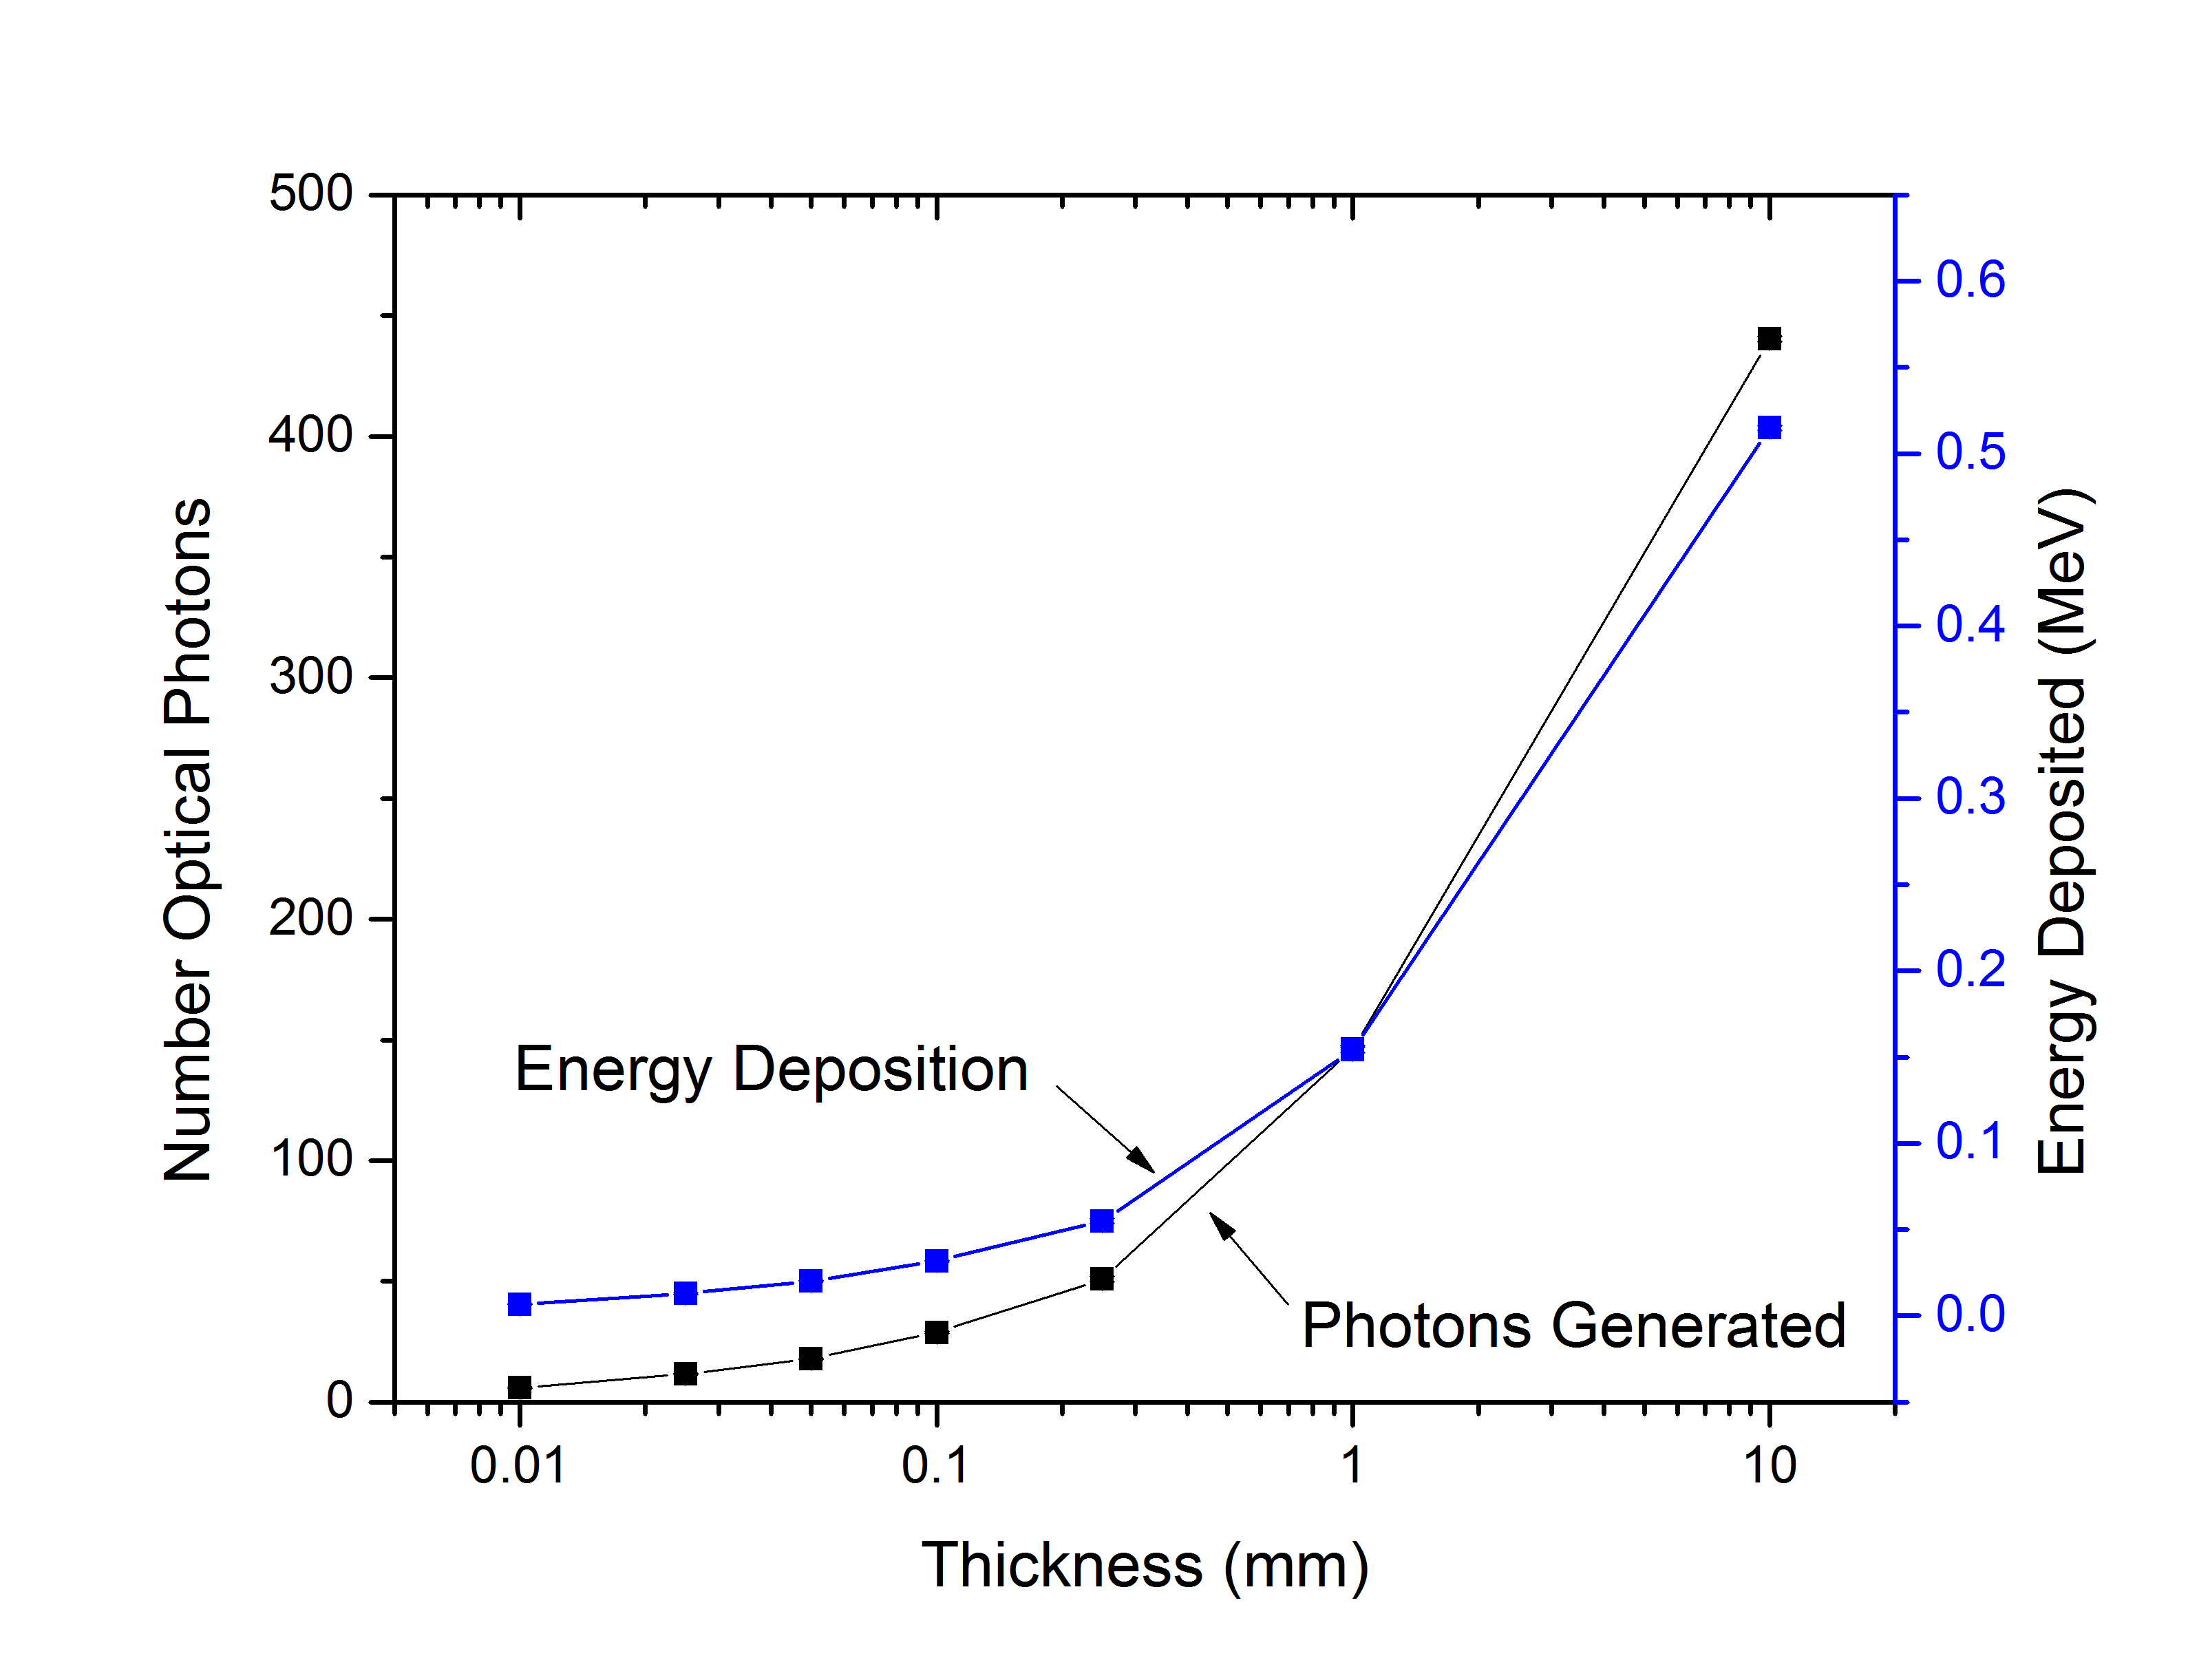
\includegraphics[width=\textwidth]{EDepLightYield_Gamma}
		\caption[Energy Deposition and Light Yield in Polystyene from Co-60 Photons]{Simulated energy deposition from gamma (\iso[60]{Co}) and the corresponding simulated light yield. \SimEDeLYGeo}
\end{figure}
\begin{figure}
 	\centering
  	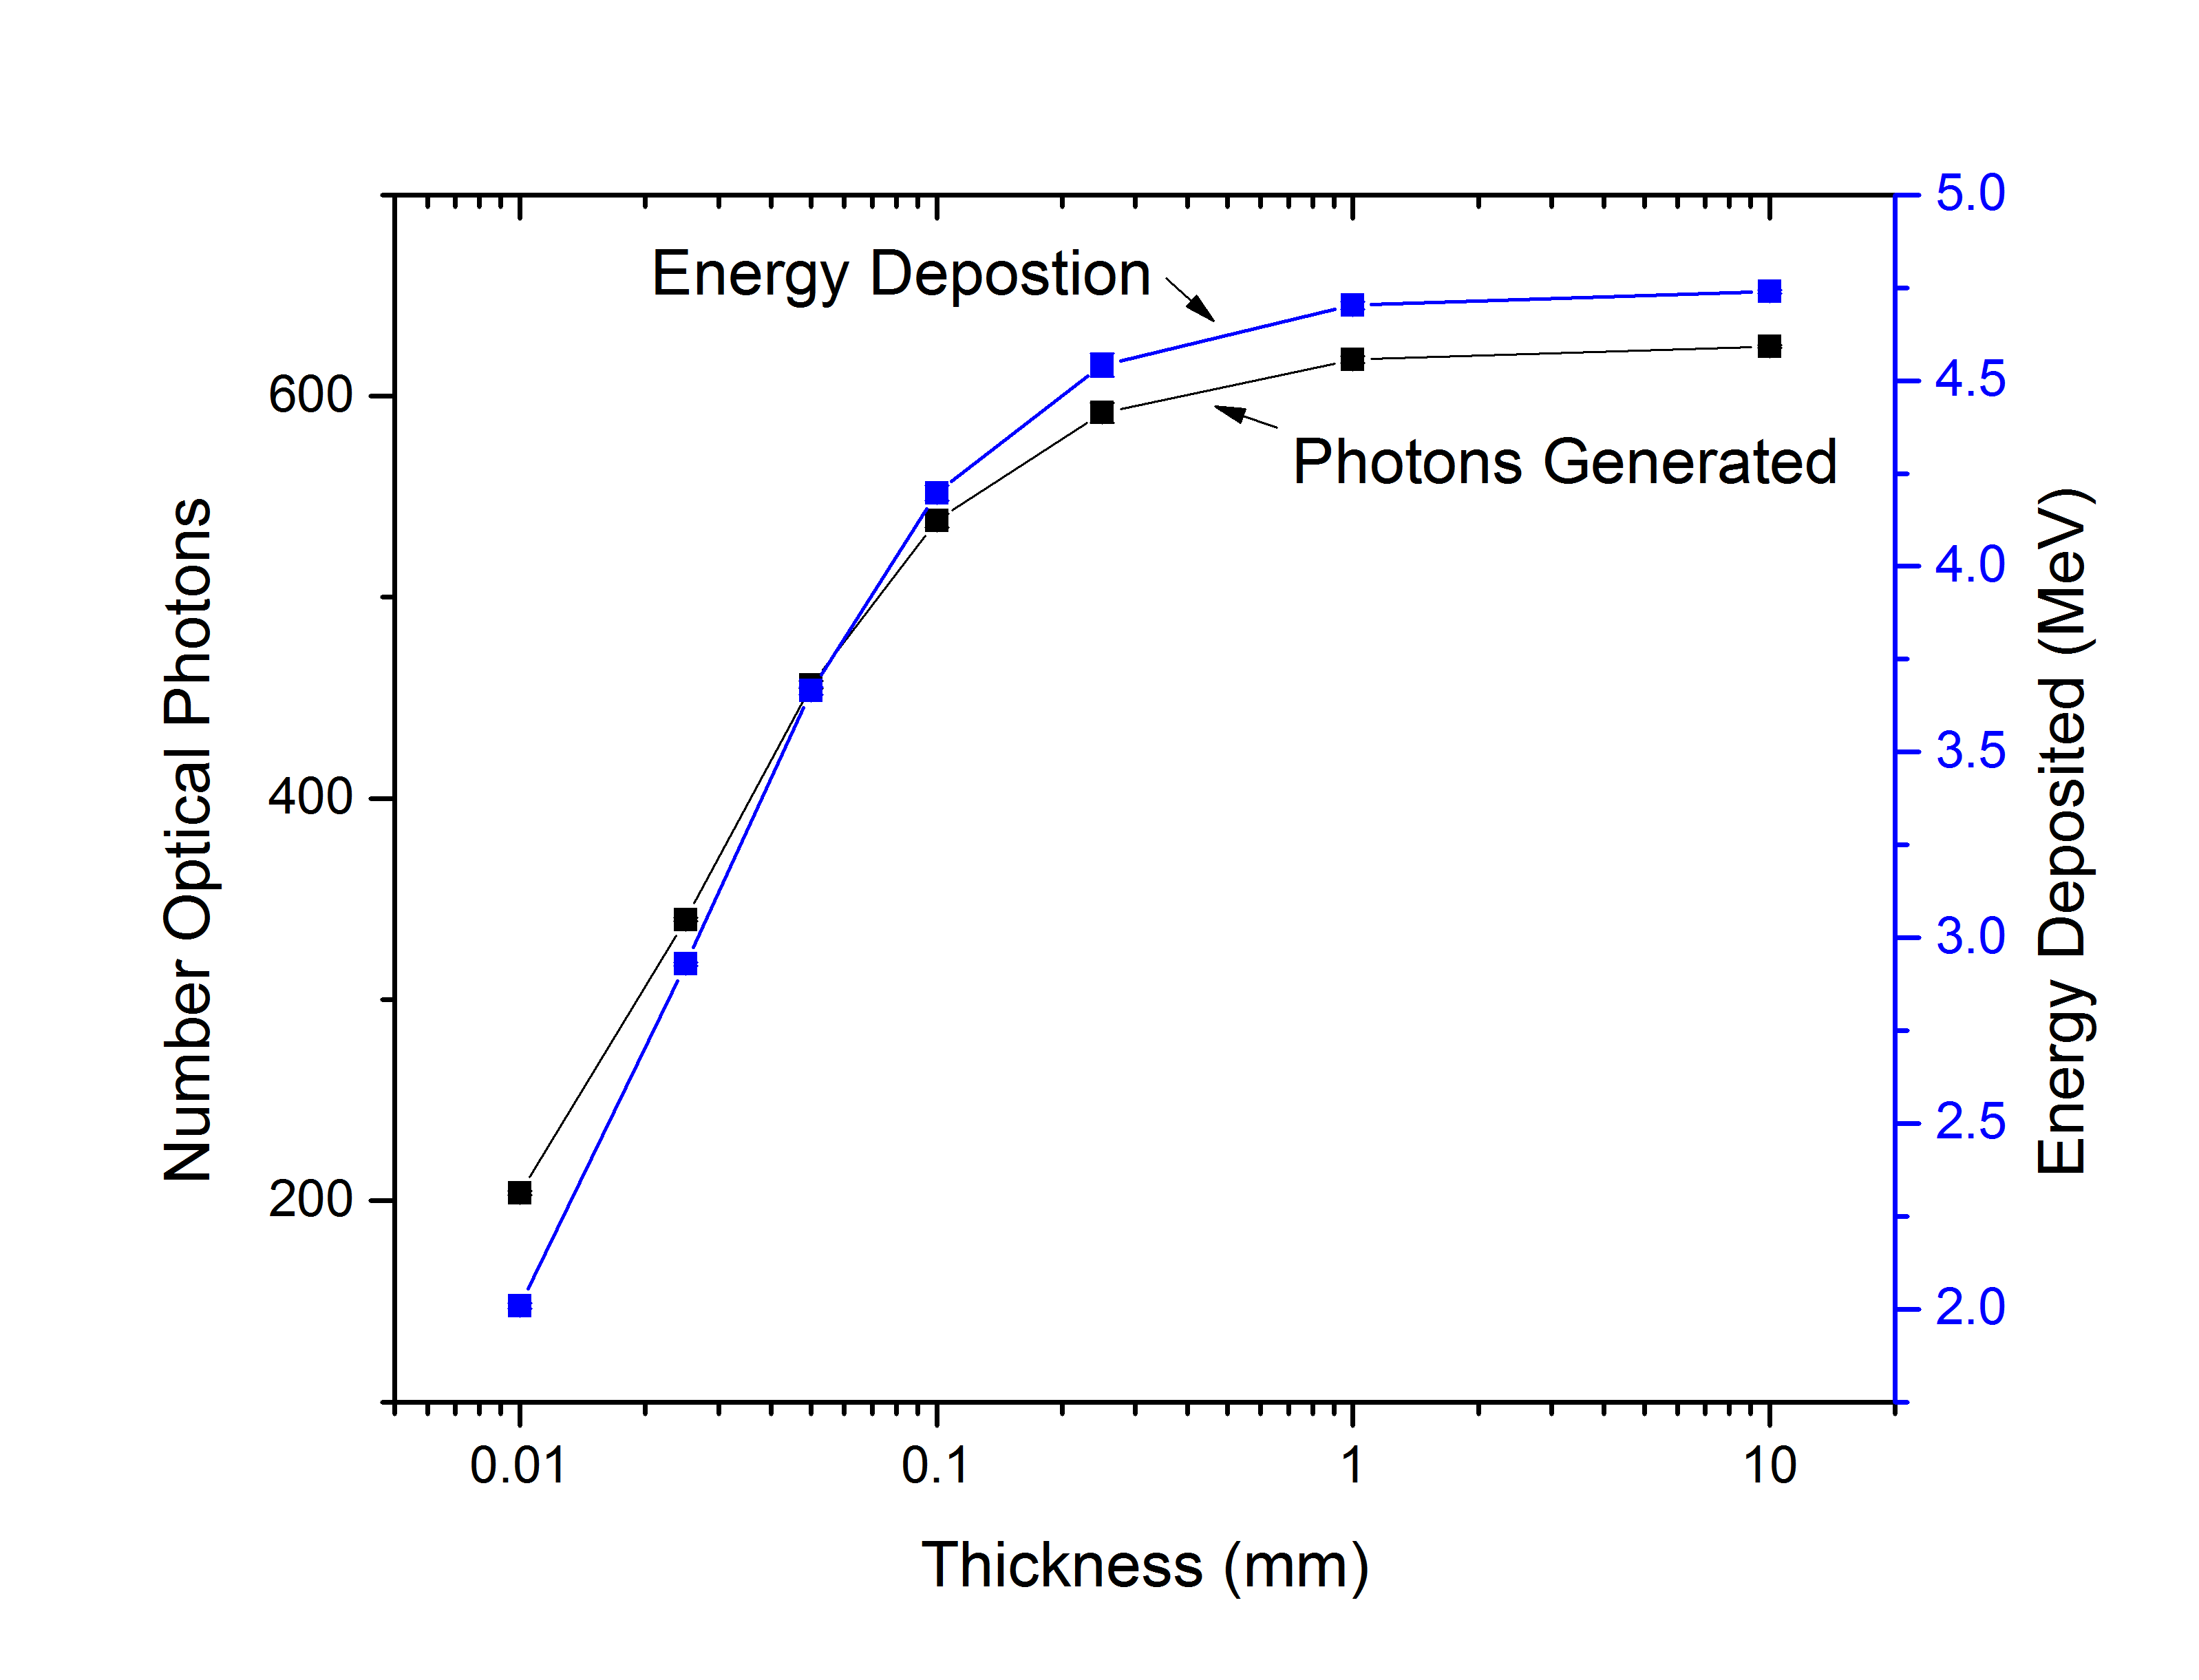
\includegraphics[width=\textwidth]{EDepLightYield_Neutron}
  	\caption[Energy Deposition and Light Yield in Polystyene from Neutrons]{Simulated energy deposition and light yield from neutron interactions.  \SimEDeLYGeo}
  \label{fig:EDepLightYield}
\end{figure}
However, it is instructive to look at the distributions of how many photons were created per event.
As the films become thicker and more of the triton energy is captured the response of the triton starts to dominate the alpha (\autoref{fig:NeutronPhotonsGenSim}), resulting in the number of photons peaking around around 650 photons for this simulated sample.
For photons, shown in \autoref{fig:GammaPhotonsGenSim}, it is observed that the distribution is flat for very thick films, but for thinner films the probability is greatly increased for an event to generate a low number of photons.
\begin{figure}
  \centering
  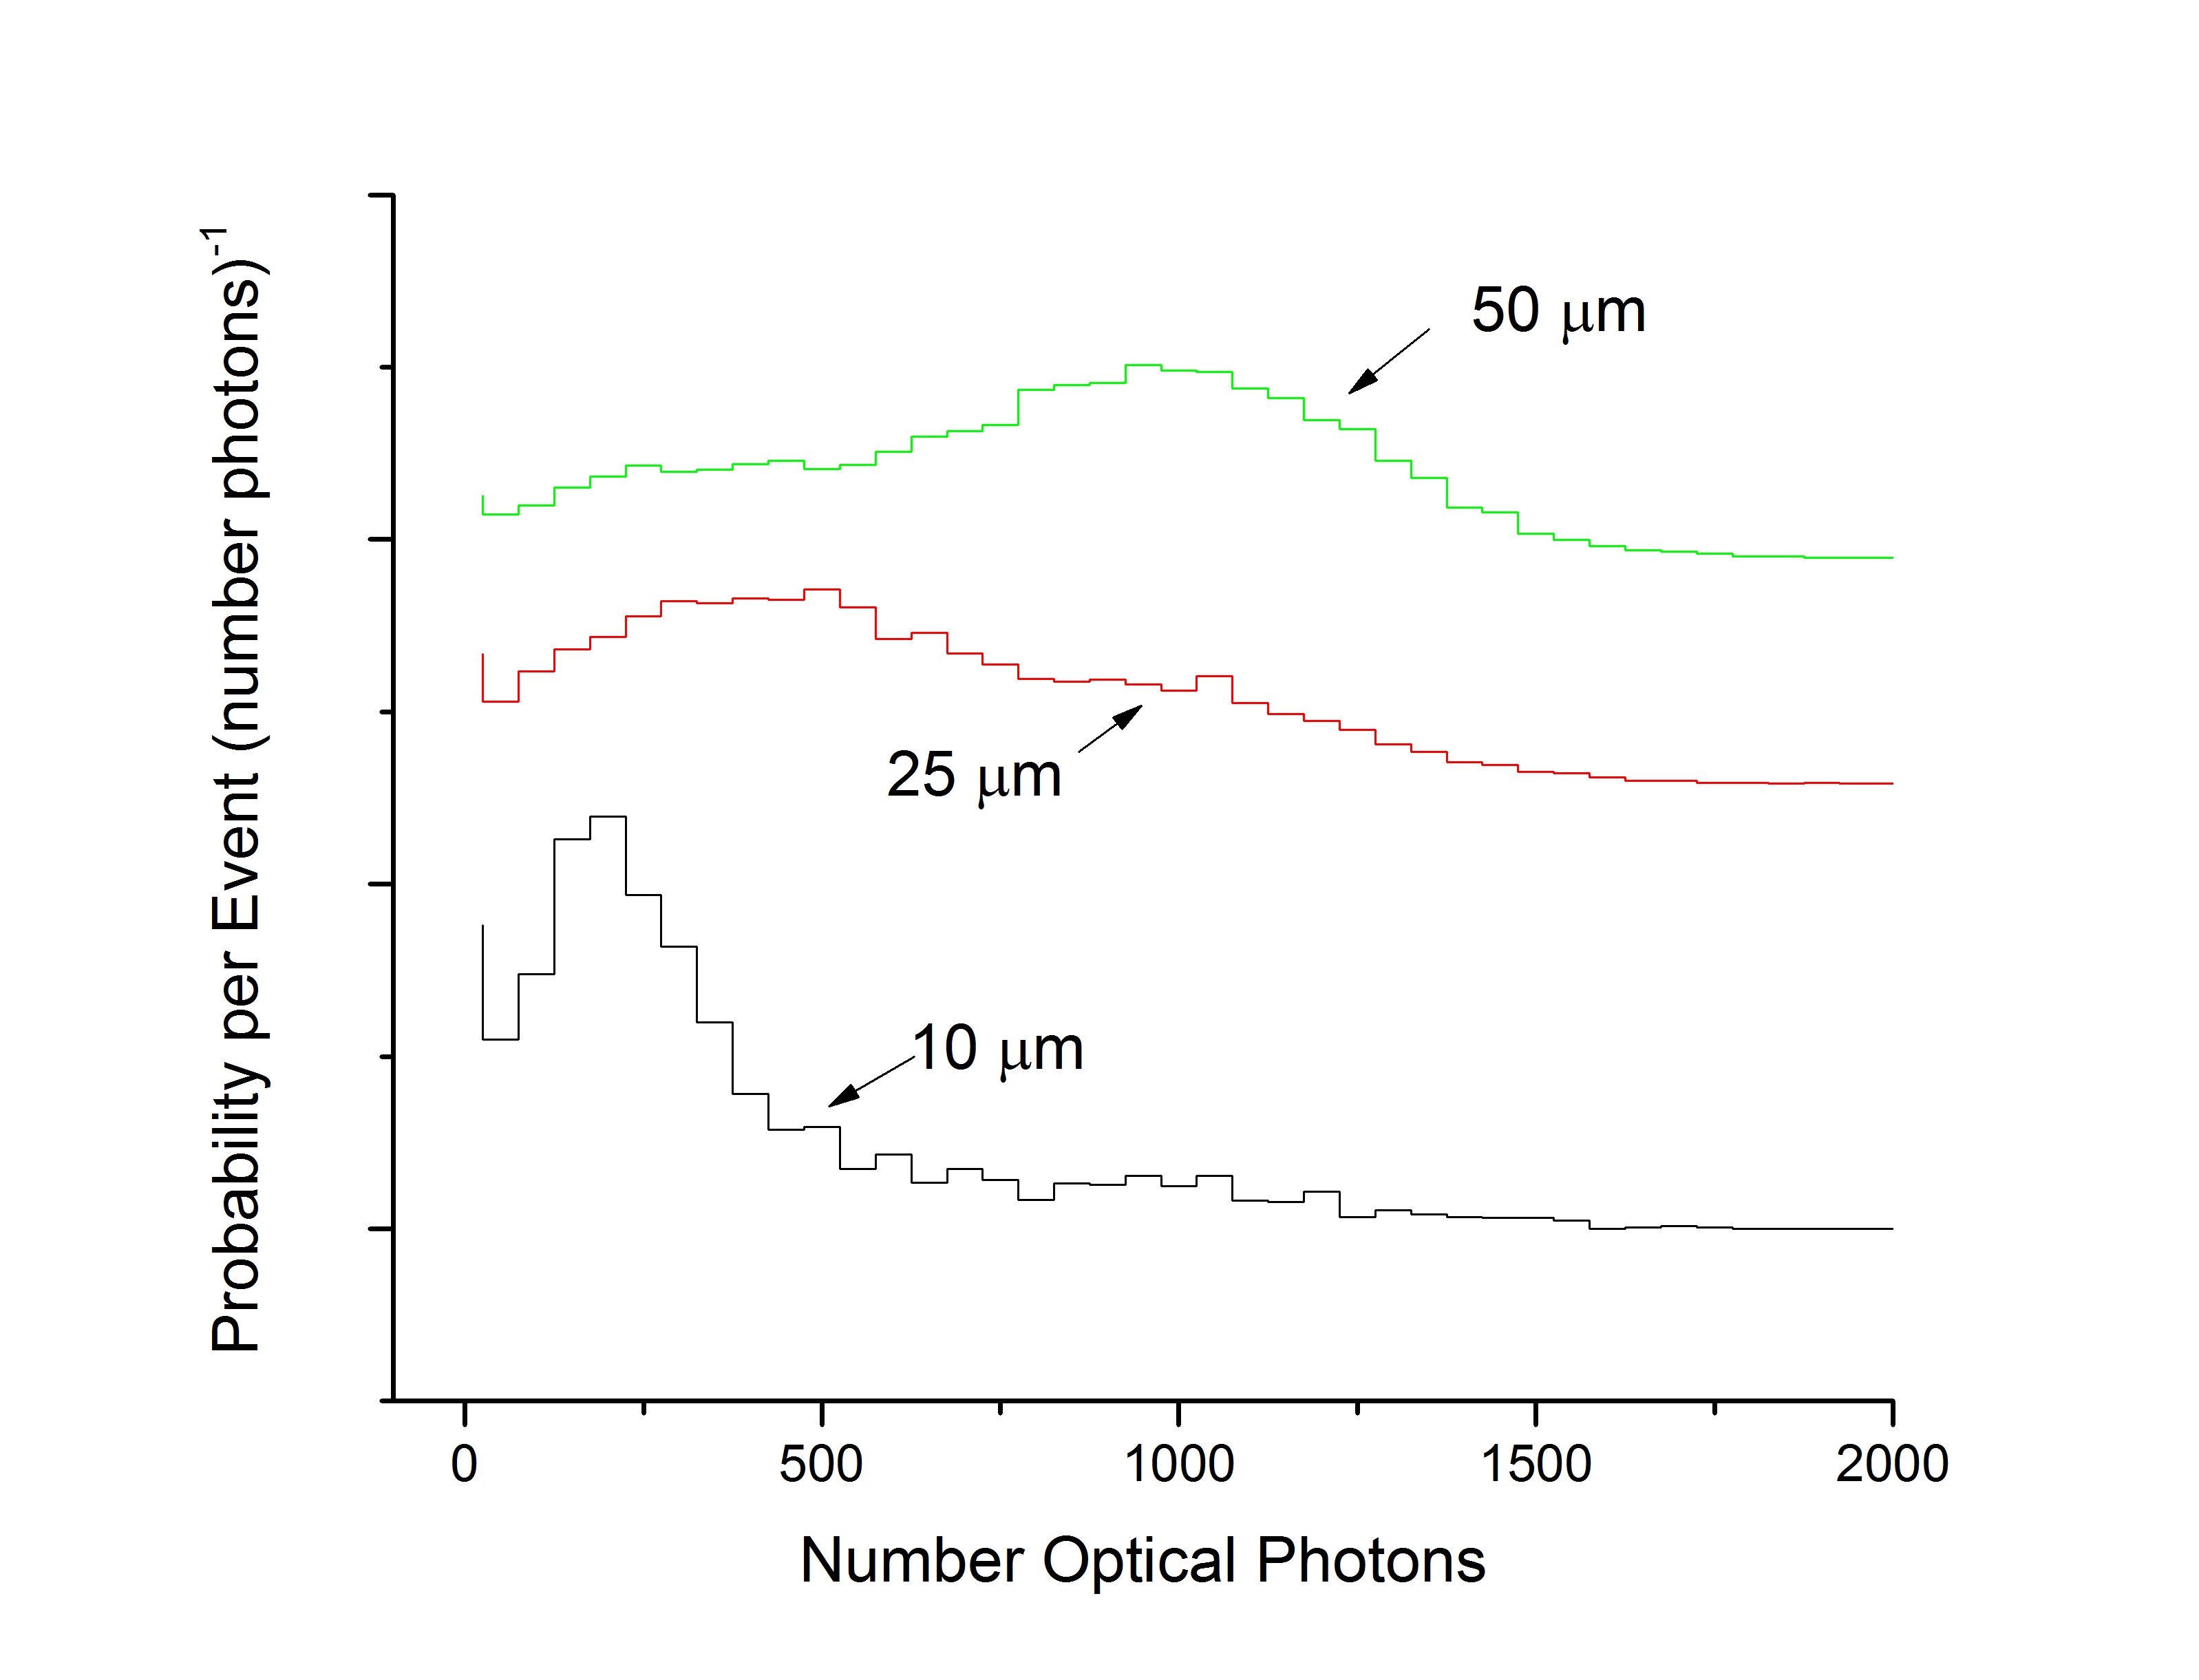
\includegraphics[width=\textwidth]{Neutron_PhotonsGenerated_Sim}
  \caption[Number of photons generated from neutron interactions]{Simulated number of photons generated from neutron interactions.  For the \SI{10}{\um} film it is observed that the majority of the photons are generated by a partial energy deposition corresponding to the alpha particle, and this effect tappers off as the films get thicker. \SimEDeLYGeo}
  \label{fig:NeutronPhotonsGenSim}
\end{figure}
\begin{figure}
  \centering
  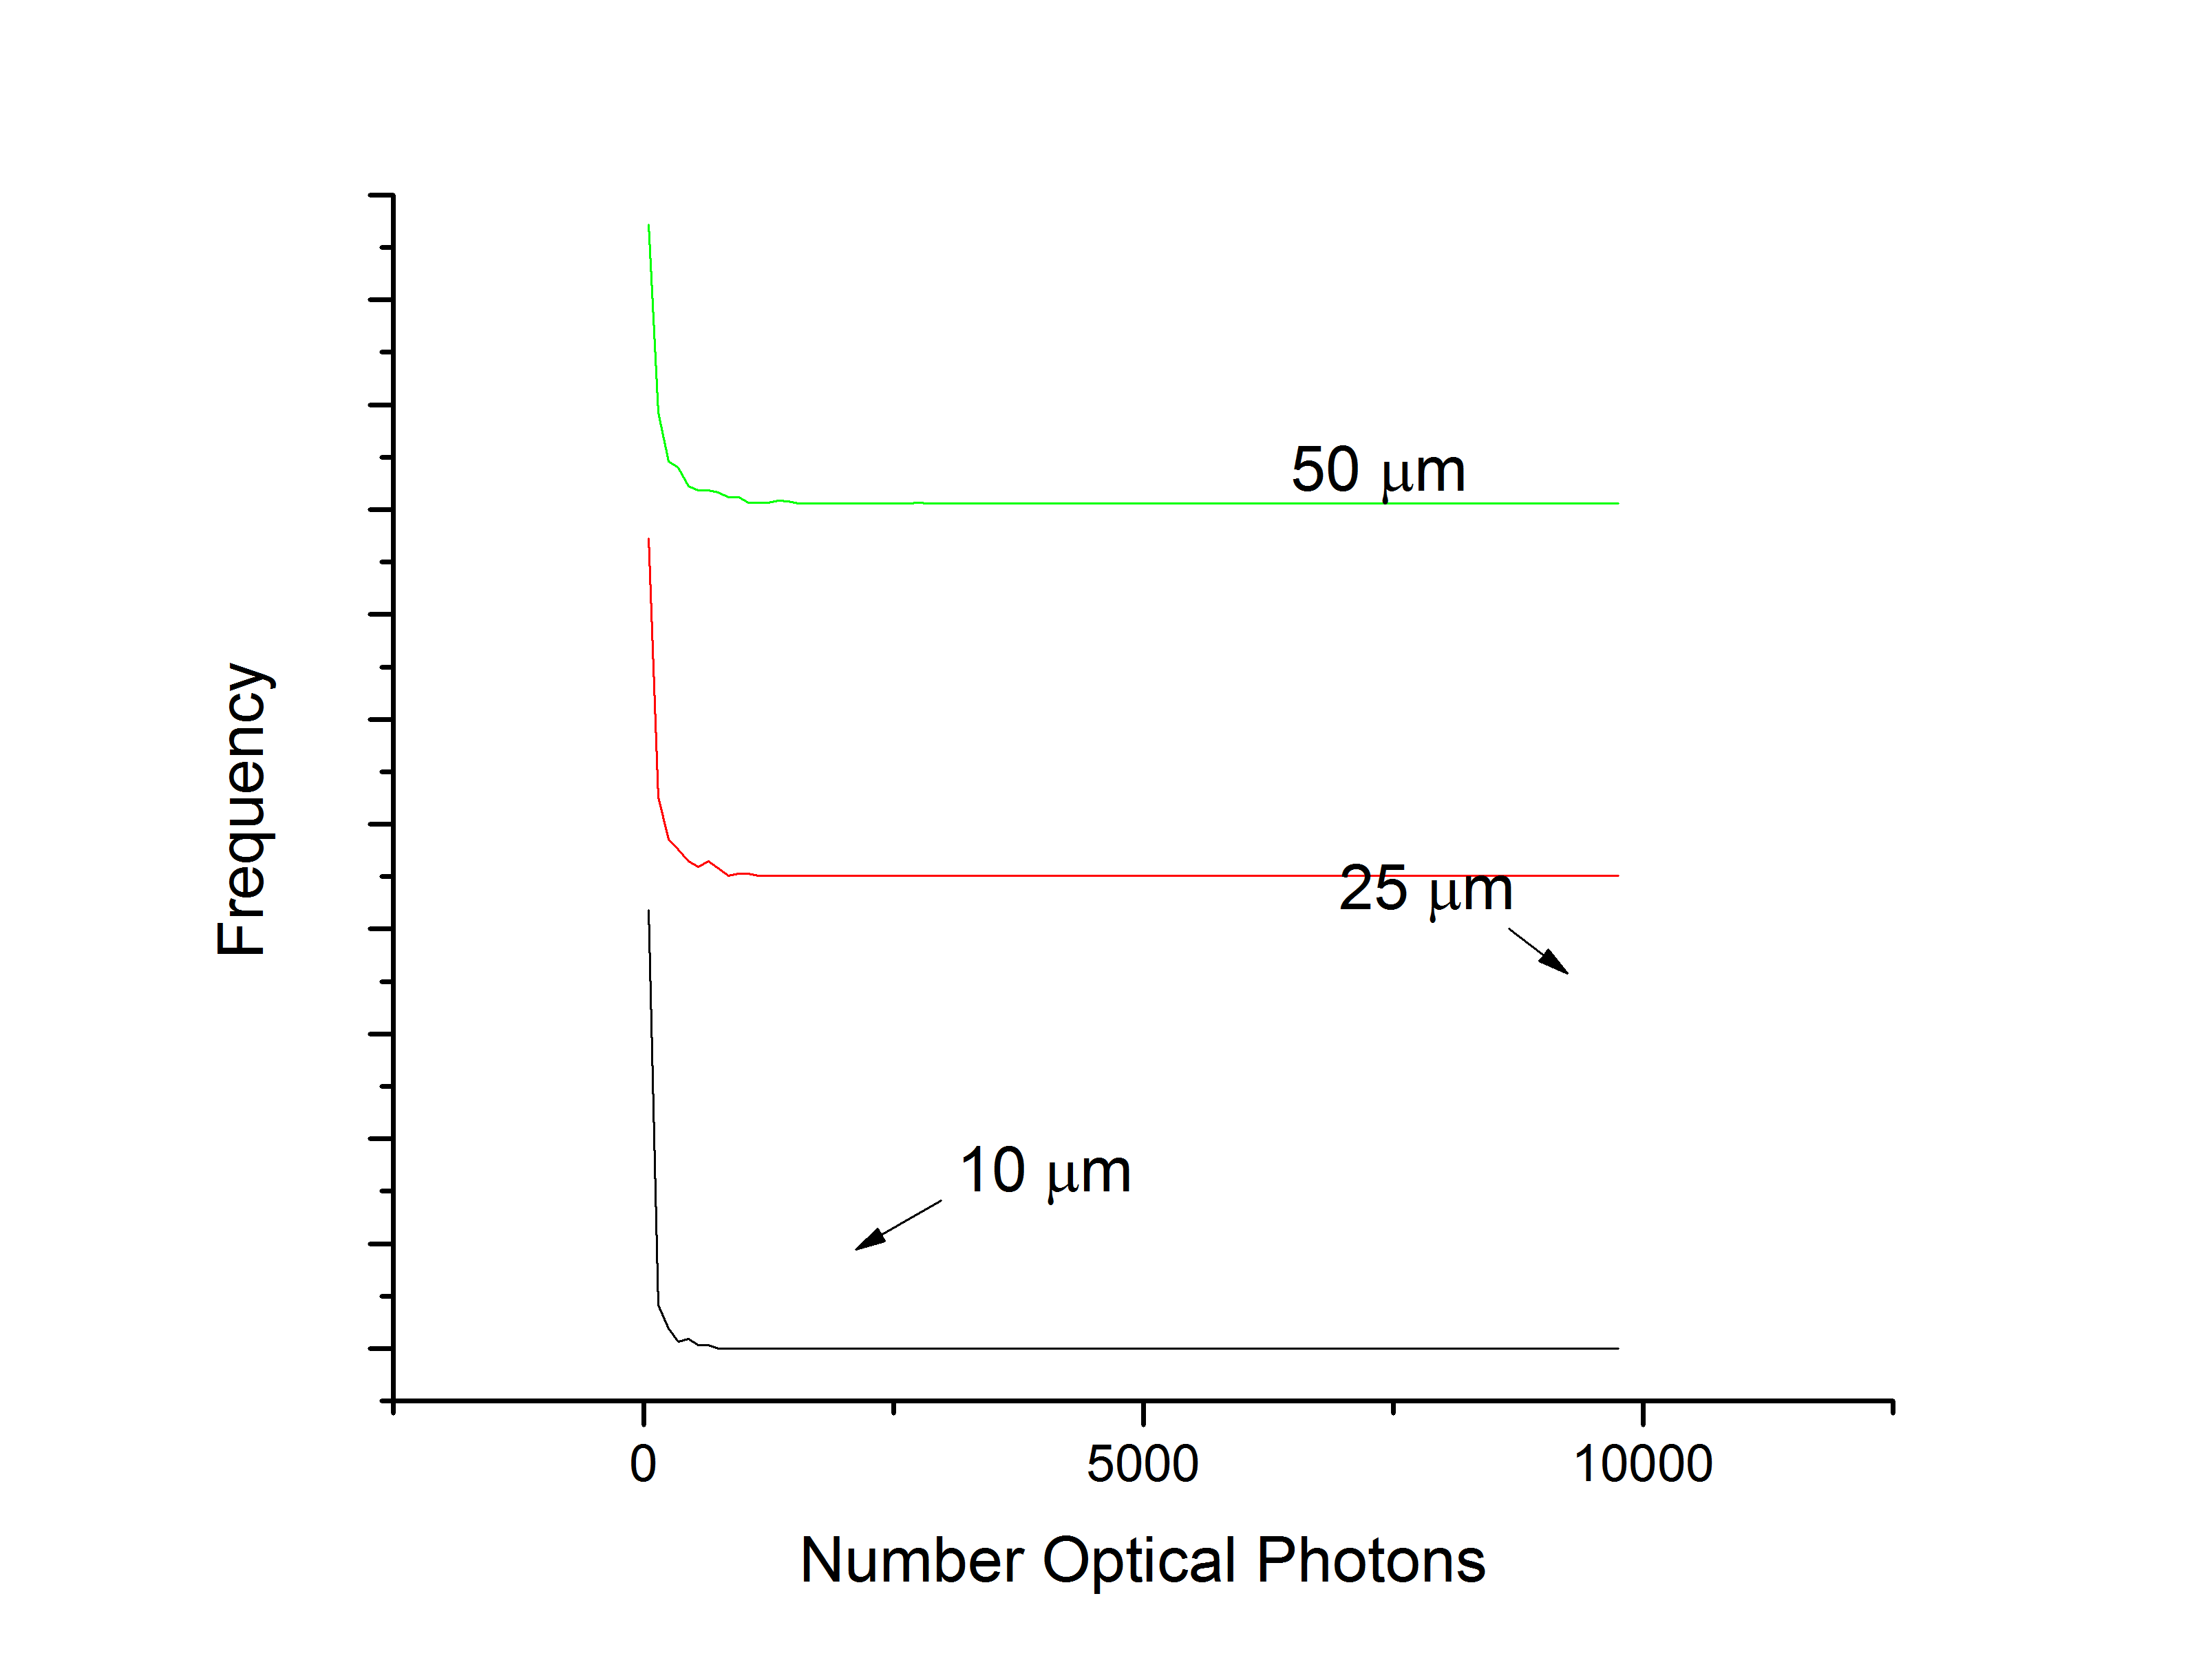
\includegraphics[width=\textwidth]{Gamma_PhotonsGenerated_Sim}
  \caption[Number of photons generated from gamma interactions]{Simulated number of photons generated from gamma interactions. Thinner films produce distrubtions that are skewed towards the left due to having less energy deposition. \SimEDeLYGeo}
  \label{fig:GammaPhotonsGenSim}
\end{figure}
\begin{figure}
  \centering
  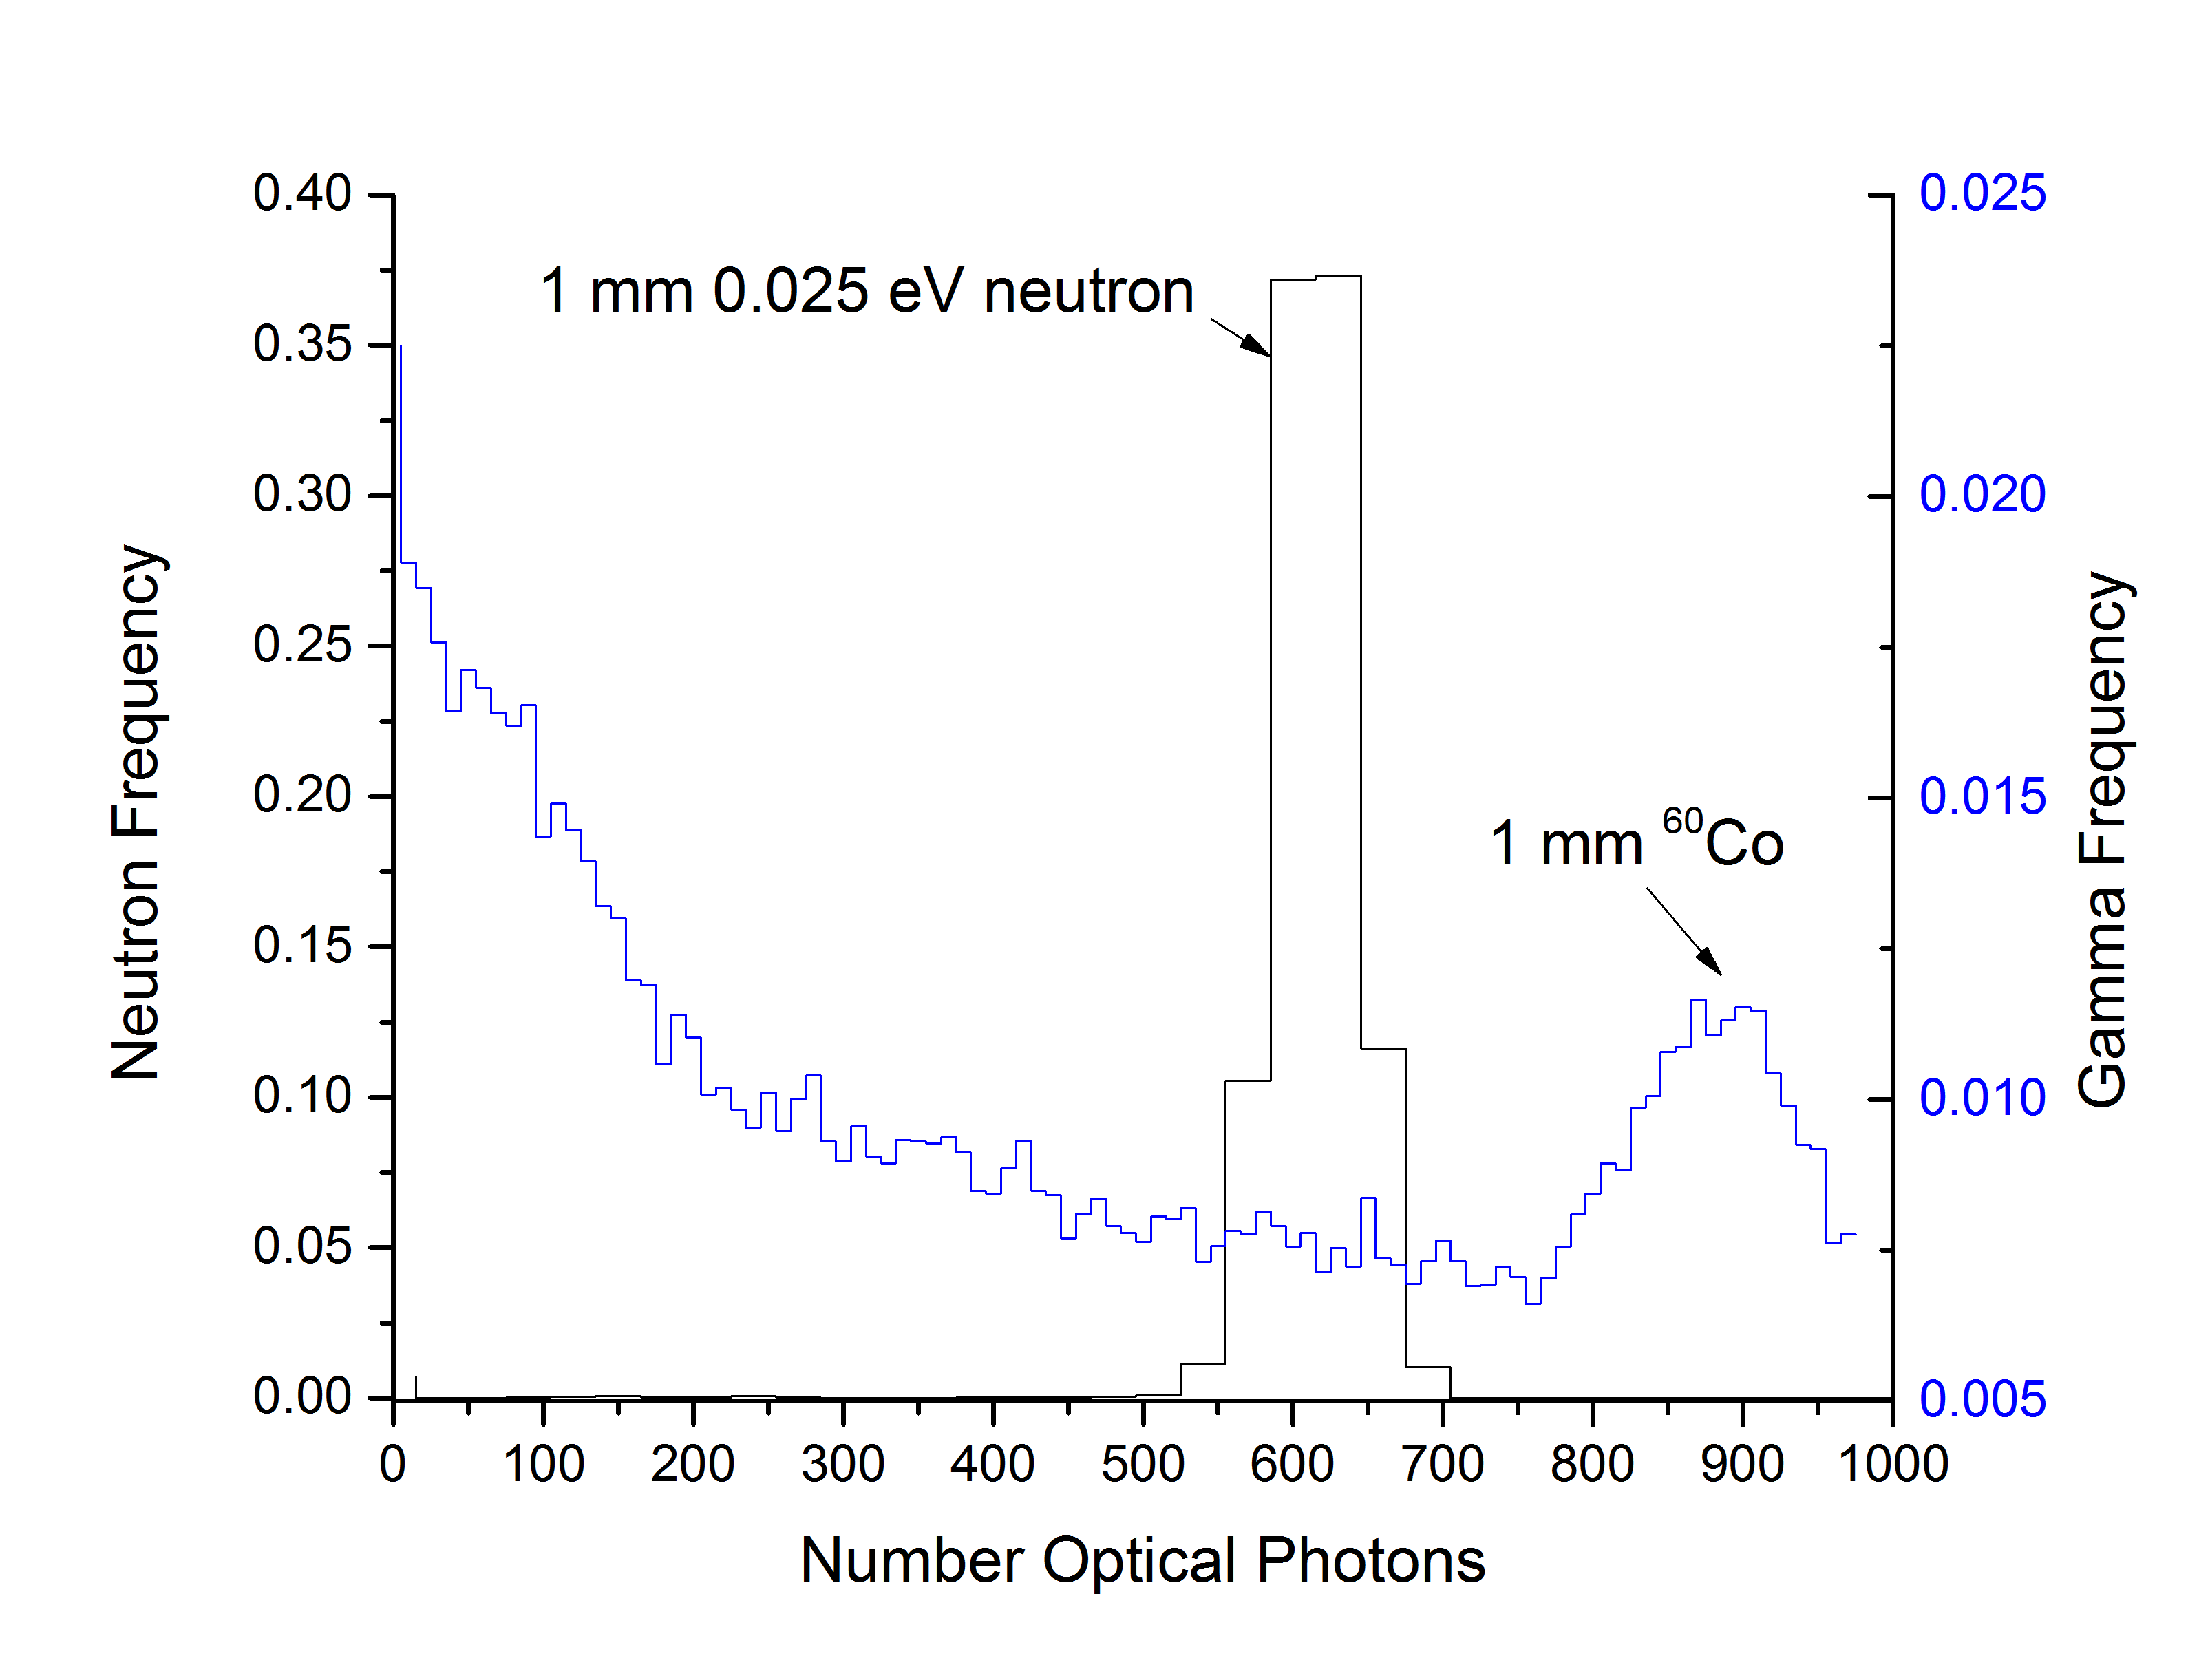
\includegraphics[width=\textwidth]{NeutronGamma_PhotonsGenerated_Sim}
  \caption[Number of photons generated of a 1 mm for neutron and gamma interactions]{Simulated number of photons generated from neutron and gamma interactions.\SimEDeLYGeo}
  \label{fig:NeutronGammaPhotonsGenSim}
\end{figure}


\section{Radiation Portal Monitor Optimization}
A single film does not have the necessary interactions to fulfill the neutron count rate criteria multiple films are necessary, and the arrangement of these films provides a design space for a replacement RPM.
In the case of the RPM, there are several design parameters that can be explored:
\begin{itemize}
  \item the neutron absorber loading of the film,
  \item the thickness of the film,
  \item the geometry of the film (cylinders or sheets), and
  \item the placement of the films.
\end{itemize}
It is expected that the loading of the film will be limited by the optical clarity, and that the thickness of the film will be determined by the optimization of the energy deposition.
Thus, of the above design parameters only the geometric placement of the films is an available optimization space.

Preliminary work by this author provided a simple design in which the detector layers are linearly placed throughout the detector volume in an alternating fashion.
The analysis of the neutron flux throughout this detector lead to a flat flux profile as shown in \autoref{fig:AltLayerThermalNeutronFraction}.
\begin{figure}
  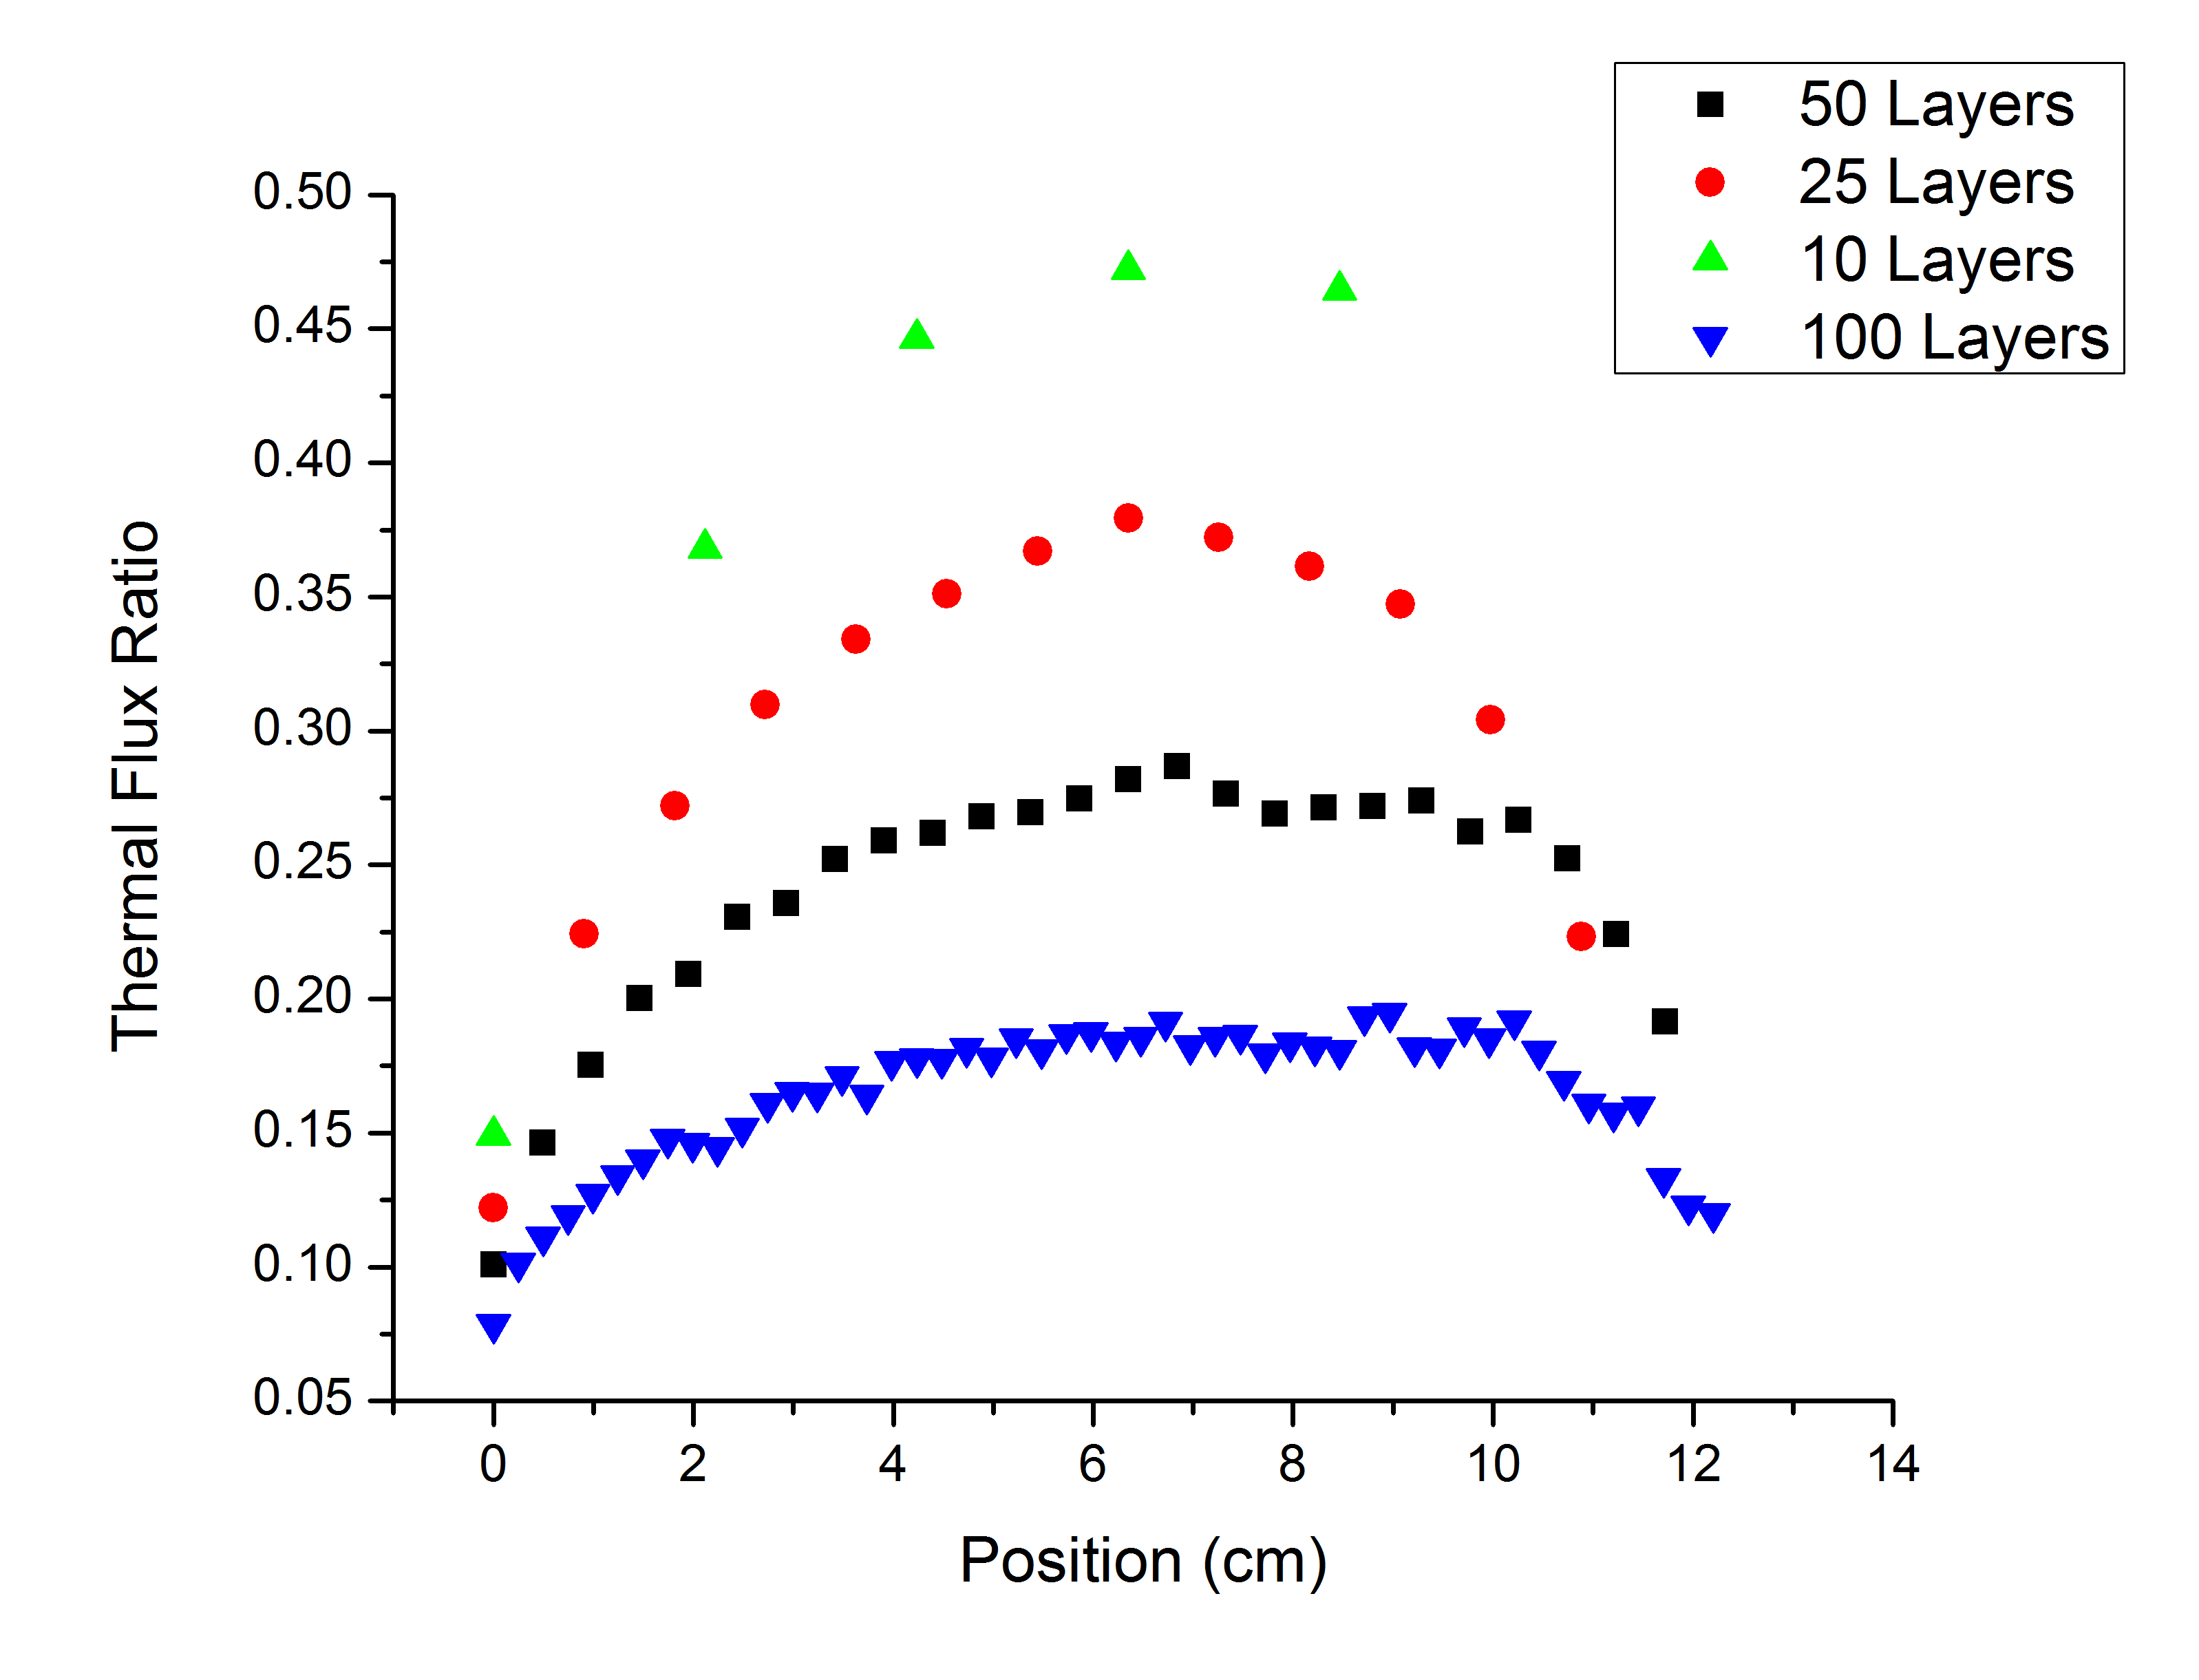
\includegraphics[width=\textwidth]{ThermalFluxRatioAltLayers}
	\caption{Fraction of the neutron flux that is thermalized through a alternating detector and moderator layered RPM.  The low thermal fluxes result in a poor utilization of the high thermal cross section of \iso[6]{Li}.}
	\label{fig:AltLayerThermalNeutronFraction}
\end{figure}
Effective utilization of the neutron flux is necessary for minimizing the amount of neutron absorber (\iso[6]{Li}) that is used in the detector.
Several different strategies can then be used to optimize the geometry to ensure effective utilization of the thermal cross section of the absorber material.

\section{Optimal Detector Geometries}

\subsection{XSDRN and MCNPX Model Comparison}
The comparison between the MCNPX simulation and the XSDRN is shown for some of the samples in \autoref{tab:10GenomeXSDRNMCNPXCompare} and \autoref{tab:20GenomeXSDRNMCNPXCompare}, where the change in rank is computed by rank of the MCNPX model versus the rank of the XSDRN model.
It is observed that the XSDRN model preformed fairly closely to the MCNPX model, but tended to over predict and favor geometries that had repeated layers and clusters.
\begin{table}
  \caption[10 Genome Length RPM Model]{10 Genome Length RPM Model Interactions rates}
  \label{tab:10GenomeXSDRNMCNPXCompare}
  \begin{tabular}{c c | c c | c}
    \toprule
    Genome & Activity & Interaction Rate & Rank Change \\
    \midrule
  0011010000& 9.30 &  3.82 & $\downarrow$ 13 \\
  0110100000 & 10.50  &  3.81 & 0 \\
  0101010000 & 10.12  & 3.79 & $\downarrow$ 7 \\
 0101100000 &  & 3.79 & $\downarrow$ 1\\
  0011100000 & 9.63 &  3.77 & $\downarrow$ 3 \\
    \bottomrule
  \end{tabular}
\end{table}
\begin{table}
  \caption[20 Genome Length RPM Model]{20 Genome Length RPM Model Interactions rates}
  \label{tab:20GenomeXSDRNMCNPXCompare}
  \begin{tabular}{c c | c c | c}
    \toprule
    Genome & Activity  & Interaction Rate & Rank Change \\
    \midrule
  00100101000000000000 & 7.77 & 3.79 & $\downarrow$ 19 \\
  00011000100000000000&  & 3.78 &  \\
  00011000010000000000& &  3.76 &  \\
  00110001000000000000 &  3.69 & $\downarrow$ 15\\
  01011010010000000000 & 23.46 & 3.66 & $\uparrow$ 1\\
    \bottomrule
  \end{tabular}
\end{table}

\subsection{Pertubations on the MCNPX Model}
Perturbations on the MCNPX were preformed in order to determine if a minimum in the search function was achieved.
A perturbation on a optimal genome is defined as taking each detector slice and translating it a half slice thickness to the left and the right. 
For example, for a five length genome a perturbation on \verb+010100+ would involve first doubling the genome to  \verb+001000100000+ and then perturbing the slices as  \verb+010000100000+, \verb+000100100000+, \verb+001001000000+, and \verb+001000010000+.
The perturbations on the length length genome increased the interaction rate from 3.81 interactions per second to 3.85 interactions per second for the optimal ten length genome, and from 3.85 interactions per second to 3.87 interactions per second.
Thus, it is determined that the genetic algorithm converged to the optimal solution.

\subsection{Optimal Geometries}
The optimal genomes are listed for 10 15, 20 length, and 30 length genomes for a minimum interaction rate of 2.5 interactions per second in \autoref{tab:GAOptRXNRate_25}, 5.0 interactions per neutron per second in \autoref{tab:GAOptRXnRate_5}, and for 7.5 interactions per second in \autoref{tab:GAOptRXNRate_75}.
It is observed that higher length genomes tended to shows a slight decrease in the total interaction rate.


\begin{table}
	\caption[Optimal geometry for 2.5 interactions per second]{Optimal genome geometries for a total minium interaction rate of 2.5 interactions per second. The detector and simulation is configured per the PNNL critera.}
	\label{tab:GAOptRXNRate_25}
	\begin{tabular}{m{7cm} m{5cm} m{2cm} }
	\toprule
	Genome & Interaction Rate per Mass \iso[6]{Li} & Mass \iso[6]{Li} \\
	\midrule
	0011010000 & 3.82 & \SI{12.6}{\gram} \\
	00100101000000000000 & 3.79 &  \SI{12.6}{\gram}  \\
	00010100001000000000000000 & 3.75 &  \SI{12.6}{\gram}  \\
	\bottomrule
	\end{tabular}
\end{table}
\begin{table}
	\caption[Optimal geometry for 5 interactions per second]{Optimal genome geometries for a total minium interaction rate of 5 interactions per second. The detector and simulation is configured per the PNNL critera.}
	\label{tab:GAOptRXNRate_5}
	\begin{tabular}{m{7cm} m{5cm} m{2cm} }
	\toprule
	Genome & Interaction Rate per Mass \iso[6]{Li} & Mass \iso[6]{Li} \\
	\midrule
	011101001000000 & 5.31 & \SI{21.0}{\gram} \\
	01011010010000000000 & 5.21& \SI{21.0}{\gram} \\
	011001001000010000000000000000 & 5.06 & \SI{21.0}{\gram} \\
	\bottomrule
	\end{tabular}
\end{table}
\begin{table}
	\caption[Optimal geometry for 7.5 interactions per second]{Optimal genome geometries for a total minium interaction rate of 7.5 interactions per second. The detector and simulation is configured per the PNNL critera.}
	\label{tab:GAOptRXNRate_75}
	\begin{tabular}{m{7cm} m{5cm} m{2cm} }
	\toprule
	Genome & Interaction Rate per Mass \iso[6]{Li} & Mass \iso[6]{Li} \\
	\midrule
	01111101110100001000 & 7.56 & \SI{41.2}{\gram} \\
	01111101010010101000 & 7.53 & \SI{41.2}{\gram} \\
	\bottomrule
	\end{tabular}
\end{table}

The neutron flux as it crosses the detector is of interest to examine the utilization of the neutrons.
\autoref{fig:20Length25MinFluxProfile} shows the flux profiles for an optimal geometry for a 20 length genome with a minimum of 2.5 interactions per second and \autoref{fig:20Length5MinFluxProfile} shows the flux profiles for a minimum of 5 interactions per second.
It is observed that the fast flux quickly decreases as the there is a build up of the thermal flux.
Once the thermal flux has reached about \SI{4E-3}{neutrons \per \cm\squared \per\second} it is advantageous to place layers of \iso[6]{Li} to reduce the thermal flux.
A build up of the thermal flux is observed after the last detector layer, and the thermal flux declines as neutrons leave the detector.
\begin{figure}
	\centering
	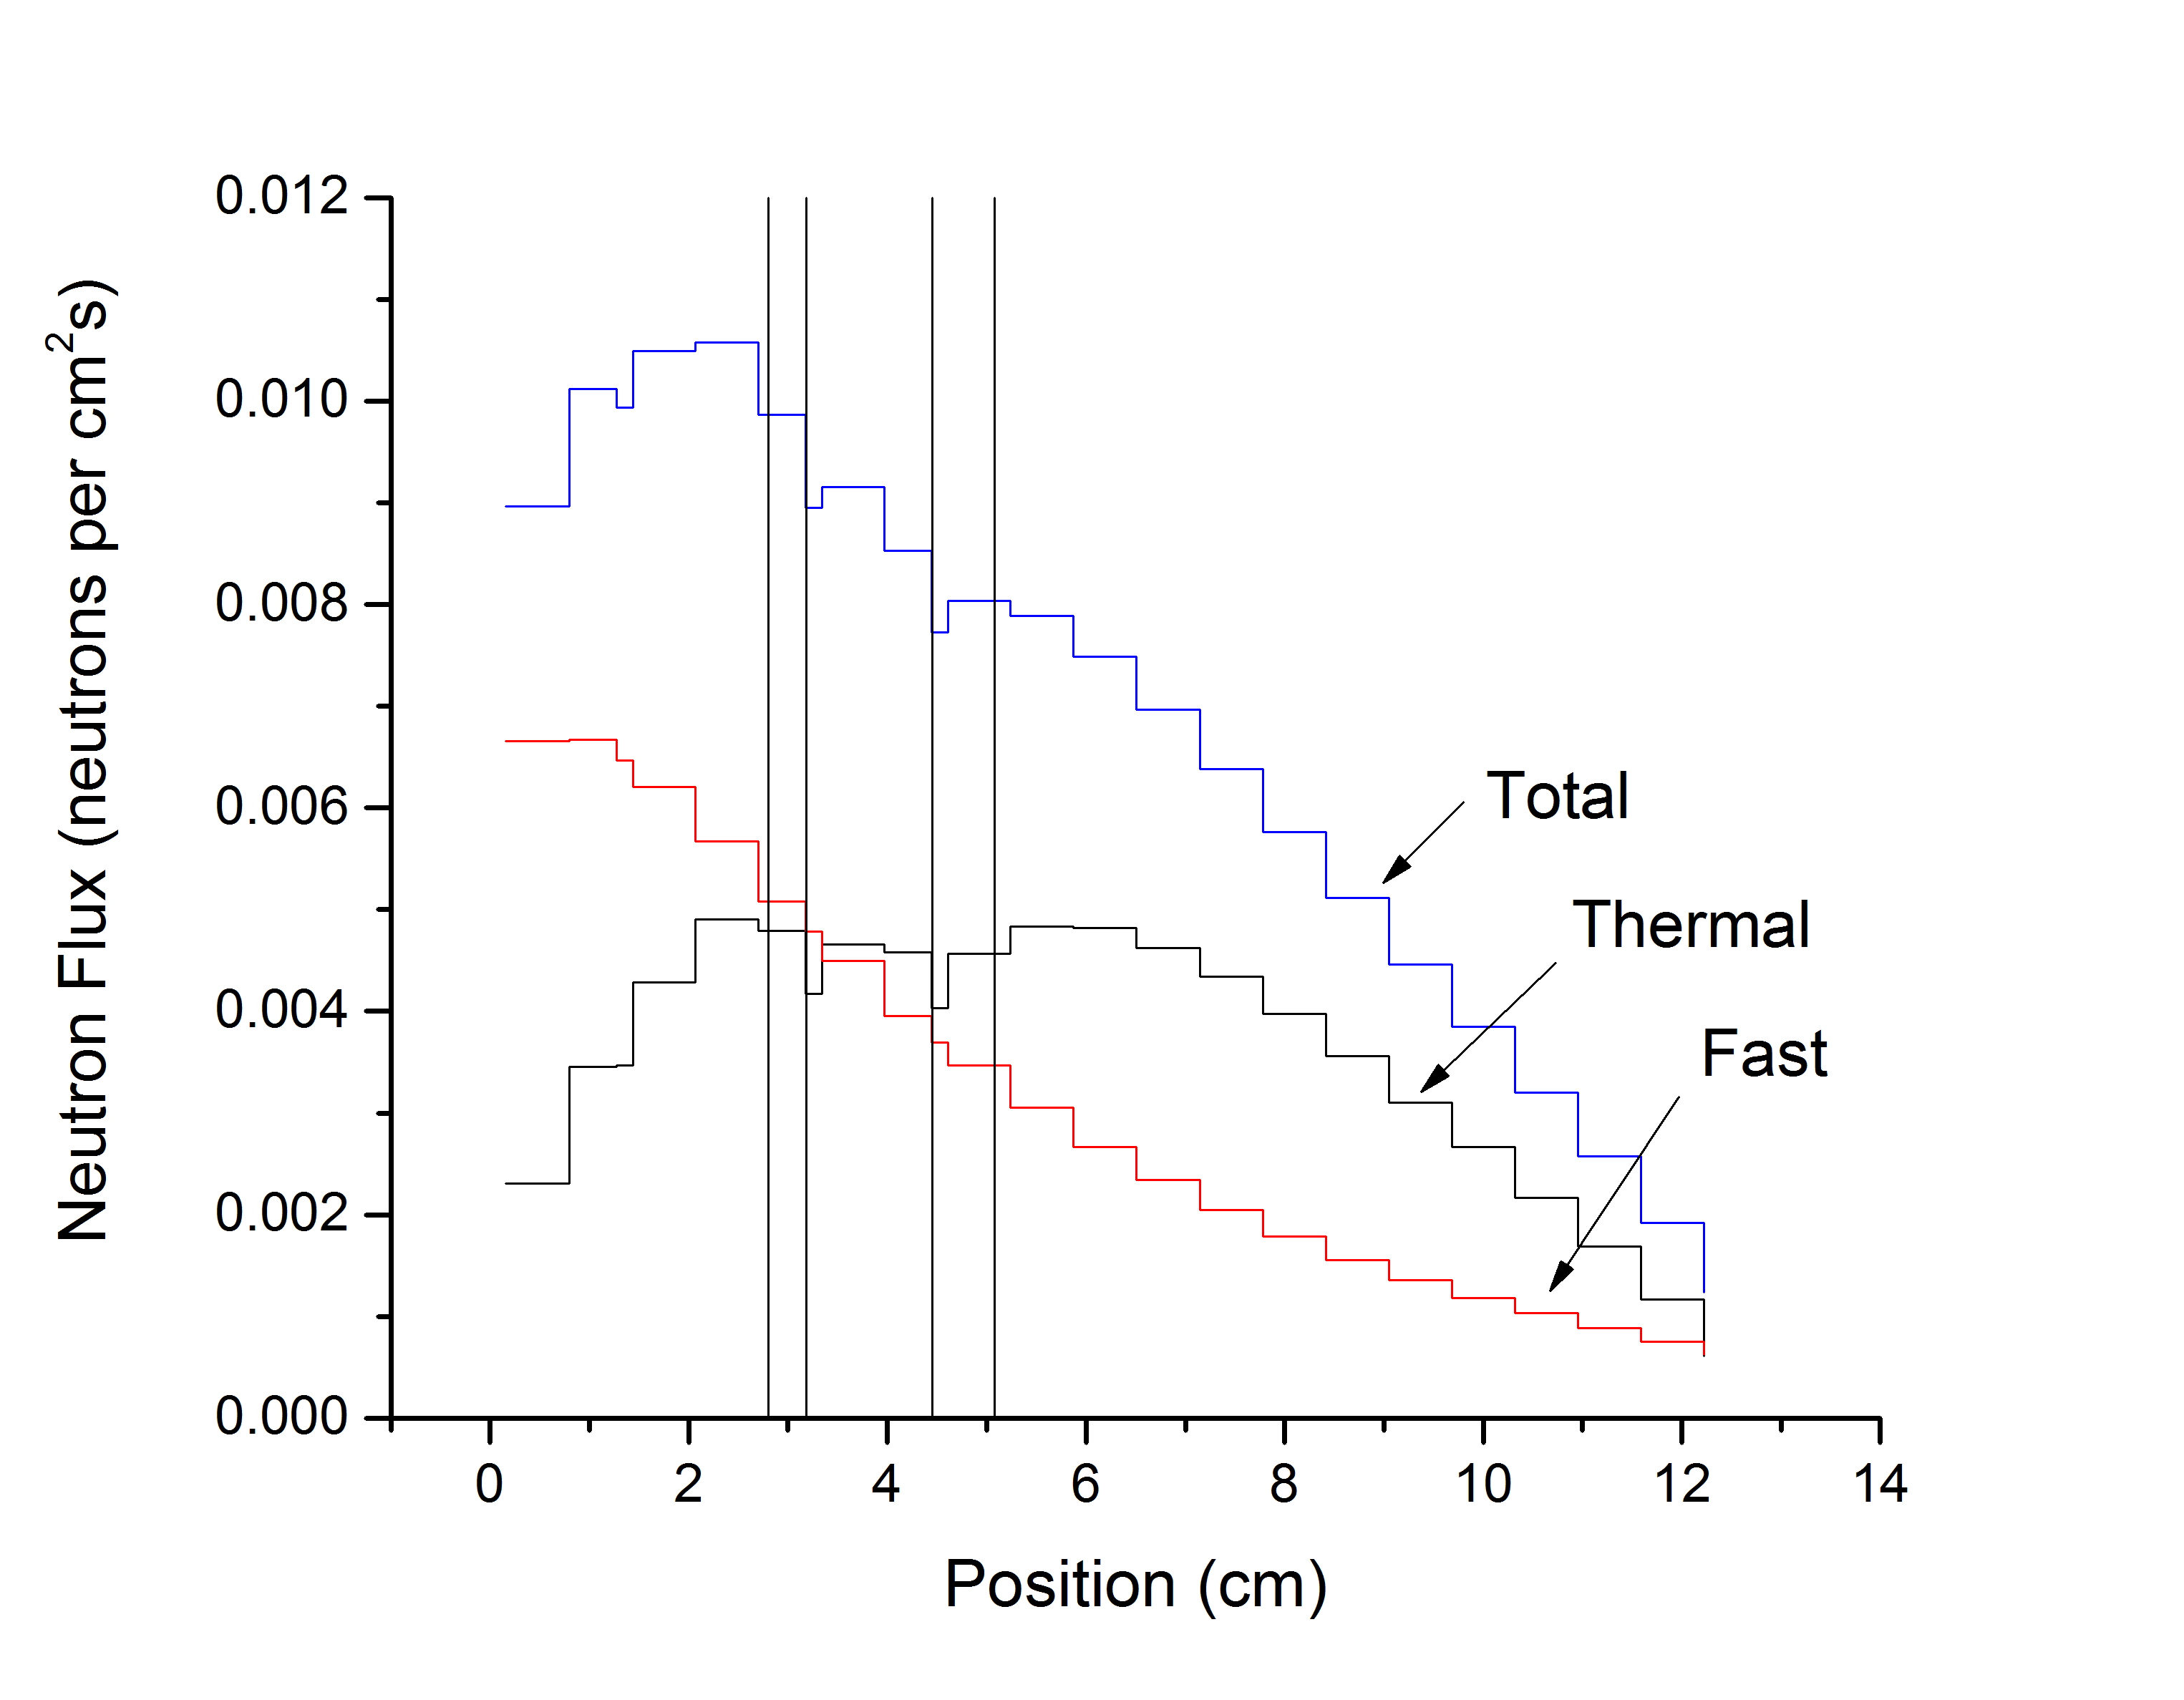
\includegraphics[width=\textwidth]{20Length25cpsMinFluxProfiles}
	\caption[Neutron Flux Profile for an Optimal 20 Length Genome, miniumn 2.5 interactions per second]{Neutron flux profile for a 20 length genome with an interaction rate of 3.82 interactions per neutron. The vertical lines represent detector slices.}
	\label{fig:20Length25MinFluxProfile}
\end{figure}
\begin{figure}
	\centering
	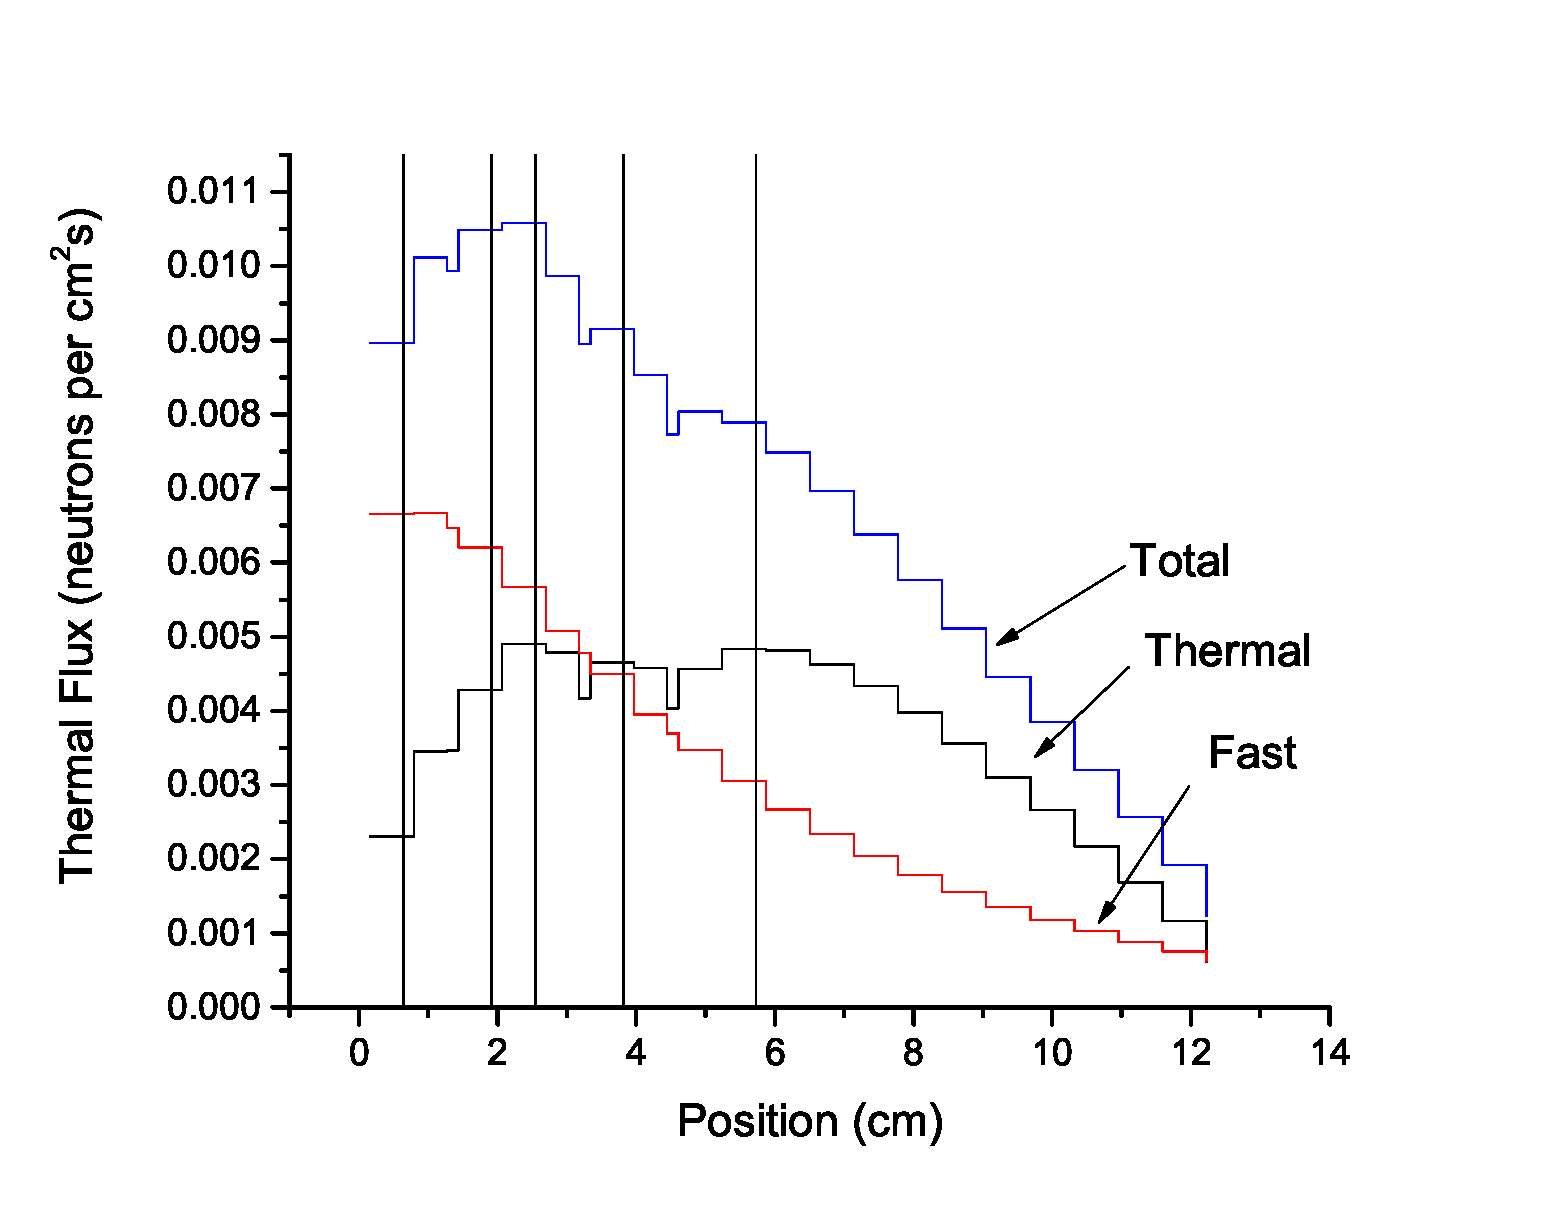
\includegraphics[width=\textwidth]{20Length5cpsMinFluxProfiles}
	\caption[Neutron Flux Profile for an Optimal 20 Length Genome, miniumn 5 interactions per second]{Neutron flux profile for a 20 length genome with an interaction rate of 5.31 interactions per neutron. The vertical lines represent detector slices.}
	\label{fig:20Length5MinFluxProfile}
\end{figure}
A physical basis of the optimal solution found by the genetic algorithm can be found by observing the form of the optimal solutions.
These solutions involve an initial moderator layer in order to ensure that all of the neutrons are thermalized to (increasing the thermal fraction by \textbf{SOME PERCENT}).
After this moderator layer a film layer is placed to utilize this neutron spectra; however not all of the thermal neutrons are captured (as the mean free path of a neutron in polyethylene is about \SI{0.37}{\cm} and thus some pass through the material) and another absorber layer is needed to capture those neutrons.  
The neutron flux is then moderated again, and additional layers of detectors are needed to capture this neutron cross section.
However, it is desirably to have a large neutron reflector in the portal monitor to reflect neutrons back into the detector slices. 
Theoretically this reflector should be as large as possible, but the limited space of the RPM provides a constraint.
A parameter study with a single detector slice between a moderator and reflector constrained by the radiation portal monitor design showed that it is desirable to have around \textbf{So much} moderator leaving the majority of the RPM to be left for the reflector.
Thus it is demonstrated that a large reflector is desired.


\section{Wrapped Polymer Cylinders}
\label{sec:WrappedCylinders}

In addition to planar detector sheets a possible replacment geoemtry could be to wrap the detector sheets around a wavelength shifting light core in concentric cylinders and replace the helium tube directly.
MCNPX simulations were completed of geometries containing two, three, and four cylinders of wrapped detector material.
It is envisioned that the detector material could be deposited on a flexible sheet and wrapped to create a cylinder, however, for simplicty a cocentric cylinder design is simulated.
The outer diamater of the cylinders were set to be two inches (\SI{2.5}{\cm}) to be a direct replacement of the existing helium three tubes.
The exact placement of the helium tubes in an RPM is not known, so the tubes were placed one-third of the way back in the detector material, and spaced equidistance apart.
The spacing of the tubes inside the radiation portal montior is described in \autoref{tab:WrappedCylinderPositions}, and shown in \autoref{fig:WrappedCylinderGeo} and \autoref{fig:WrappedCylinderPos}.
\begin{figure}
  \centering
  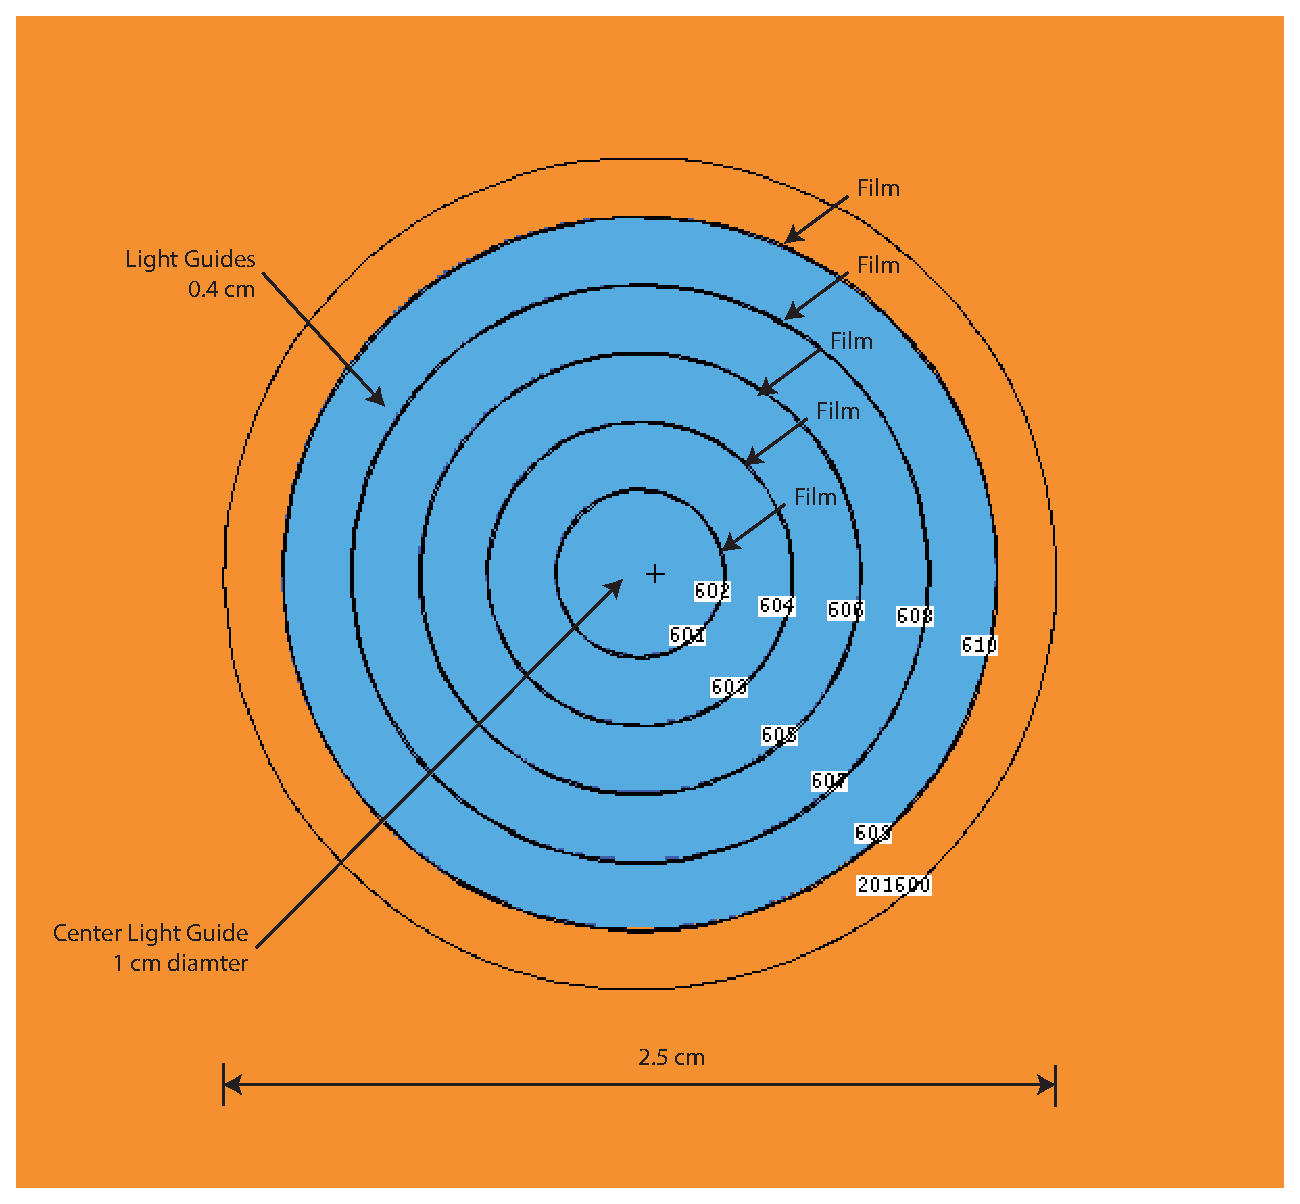
\includegraphics[width=\textwidth]{WrappedGeoCylinder_WrappedCylinder.eps}
  \caption[Rendering of Wrapped Cylinder Geometry]{MCNPX Rendering of a wrapped cylinder.  There is a \SI{1}{\cm} diamter inner light guide surrounded by films seperated by \SI{0.4}{\cm} thick light guides.}
  \label{fig:WrappedCylinderGeo}
\end{figure}
\begin{figure}
  \centering
  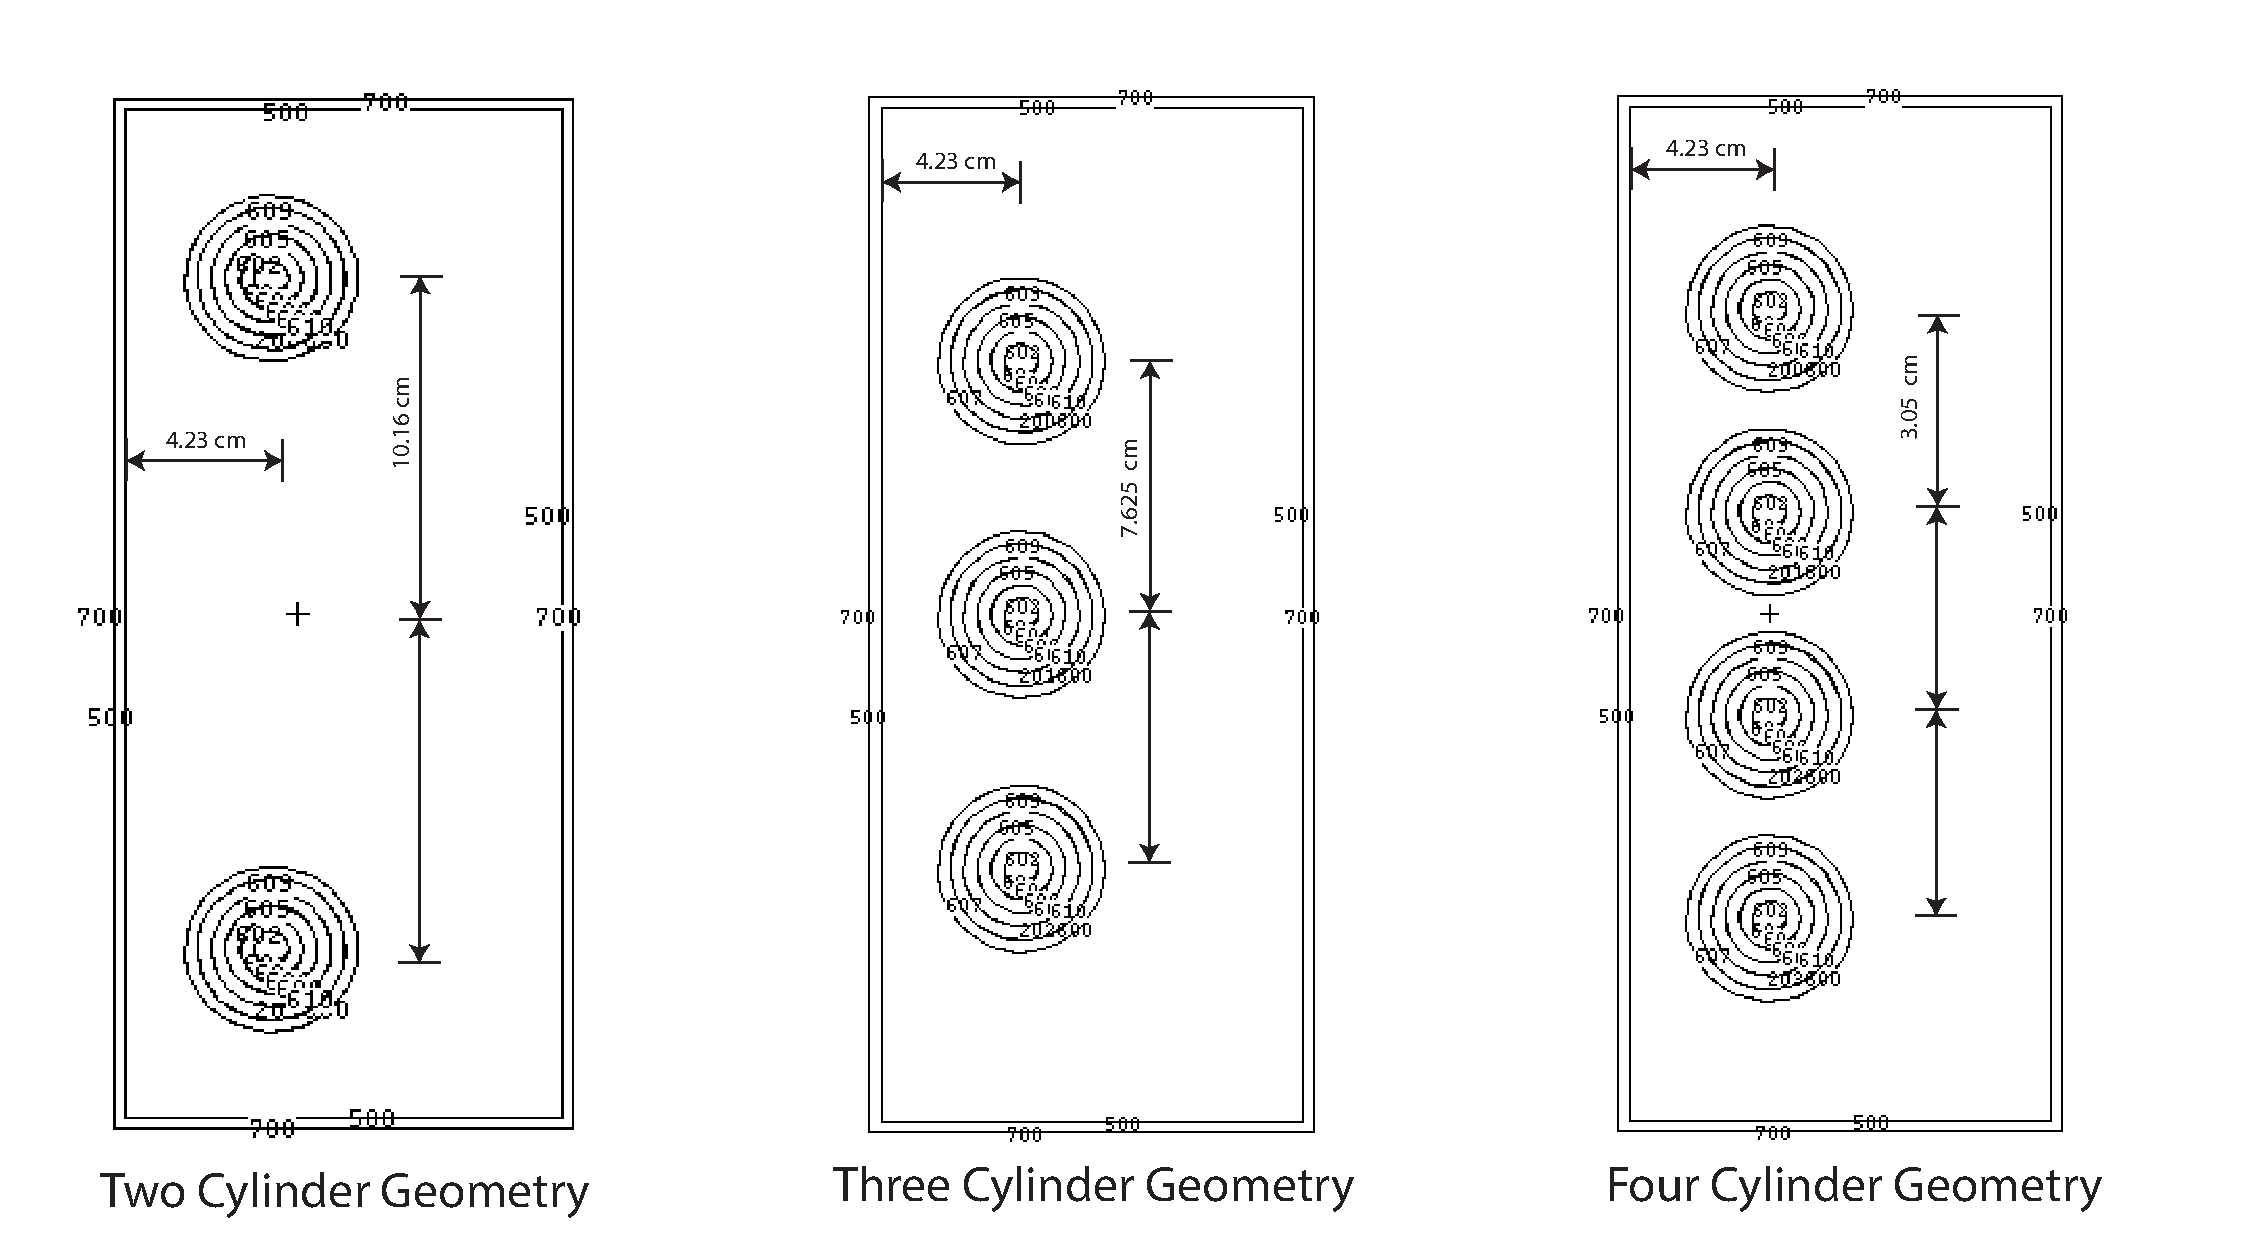
\includegraphics[width=\textwidth]{WrappedGeoCylinder_WrappedCylinderPositions.eps}
  \caption[Positions of Wrapped Cylinders in RPM Cabinet]{MCNPX Rendering of wrapped cylinders placed in an RPM8 Cabinet.}
  \label{fig:WrappedCylinderPos}
\end{figure}
The thickness of the RPM (\SI{12.7}{\cm}) corresponds to the x dimension, where the front of the detector is at x equals \SI{0.0}{\cm}.
The width of the RPM cabinet extends from \SI{-15.25}{\cm} to \SI{15.25}{\cm}, where a y corridante of zero is on the midline of the detector width.
\begin{table}
  \caption[Wrapped Cylinder Positions]{Positions of the wrapped cylinders in the RPM. The thickness of the RPM corresponds to the x dimension, and the width of the RPM cabinet extends from \SI{-15.25}{\cm} to \SI{15.25}{\cm}}
  \label{tab:WrappedCylinderPositions}
  \begin{tabular}{m{2cm} | m{3cm} m{4cm} }
    \toprule
    Number Cylinders & x corridnate & y corridinate \\
    \midrule
    2 & \SI{4.23}{\cm} & $\pm$ \SI{10.16}{\cm} \\
    3 & \SI{4.23}{\cm} & \SI{0}{\cm}, $\pm$ \SI{7.625}{\cm} \\
    4 & \SI{4.23}{\cm} & $\pm$ \SI{3.05}{\cm}, $\pm$ \SI{9.15}{\cm} \\
    \bottomrule
  \end{tabular}
\end{table}
\begin{table}
  \caption[Two Wrapped Cylinders Interaction Rate]{MCNPX simulated interaction rate of two wrapped cylinders of polymer loaded \iso[6]{LiF} in the RPM8 footprint}
  \label{tab:TwoCylinderResults}
	\begin{tabular}{m{2cm} >{\centering\arraybackslash} m{2cm} >{\centering\arraybackslash} m{2cm} >{\centering\arraybackslash} m{4cm} >{\centering\arraybackslash} m{4cm} }
	\toprule
    Polymer& Fraction \iso[6]{LiF} & Mass \iso[6]{Li}& Count Rate  & count rate per mass \\
           &                       &  \centering{\si{\gram}} & \si{\cps\per\ng} \iso[255]{Cf}  & \si{\cps\per\ng \iso[252]{Cf}\per\gram} \\
    \midrule
    PS     &  0.10  &  2.401 &   1.321 $\pm$   0.03 &   0.550 \\ 
    PS     &  0.20  &  4.798 &   1.852 $\pm$   0.04 &   0.386 \\
    PS     &  0.30  &  7.192 &   2.160 $\pm$   0.04 &   0.300 \\
    PEN    &  0.10  &  2.384 &   1.325 $\pm$   0.03 &   0.556 \\
    PEN    &  0.20  &  4.769 &   1.841 $\pm$   0.04 &   0.386 \\
    PEN    &  0.30  &  7.154 &   2.157 $\pm$   0.04 &   0.302 \\ 
    \bottomrule
  \end{tabular}
\end{table}

\begin{table}
  \caption[Three Wrapped Cylinders Interaction Rate]{MCNPX simulated interaction rate of three wrapped cylinders of polymer loaded \iso[6]{LiF} in the RPM8 footprint}
  \label{tab:ThreeCylinderResults}
	\begin{tabular}{m{2cm} >{\centering\arraybackslash} m{2cm} >{\centering\arraybackslash} m{2cm} >{\centering\arraybackslash} m{4cm} >{\centering\arraybackslash} m{4cm} }
	\toprule
    Polymer& Fraction \iso[6]{LiF} & Mass \iso[6]{Li}& Count Rate  & count rate per mass \\
           &                       &  \centering{\si{\gram}} & \si{\cps\per\ng} \iso[255]{Cf}  & \si{\cps\per\ng \iso[252]{Cf}\per\gram} \\
    \midrule
    PS     &  0.10  &  2.401 &   1.482 $\pm$  0.02 &   0.617 \\
    PS     &  0.20  &  4.798 &   2.240 $\pm$  0.03 &   0.467 \\
    PS     &  0.30  &  7.192 &   2.706 $\pm$  0.04 &   0.376 \\
    PEN    &  0.10  &  2.384 &   1.368 $\pm$  0.02 &   0.574 \\
    PEN    &  0.20  &  4.769 &   2.119 $\pm$  0.03 &   0.444 \\
    PEN    &  0.30  &  7.154 &   2.608 $\pm$  0.04 &   0.365 \\
    \bottomrule
  \end{tabular}
\end{table}

\begin{table}
  \caption[Four Wrapped Cylinders Interaction Rate]{MCNPX simulated interaction rate of four wrapped cylinders of polymer loaded \iso[6]{LiF} in the RPM8 footprint}
  \label{tab:FourCylinderResults}
	\begin{tabular}{m{2cm} >{\centering\arraybackslash} m{2cm} >{\centering\arraybackslash} m{2cm} >{\centering\arraybackslash} m{4cm} >{\centering\arraybackslash} m{4cm} }
	\toprule
    Polymer& Fraction \iso[6]{LiF} & Mass \iso[6]{Li}& Count Rate  & count rate per mass \\
           &                       &  \centering{\si{\gram}} & \si{\cps\per\ng} \iso[255]{Cf}  & \si{\cps\per\ng \iso[252]{Cf}\per\gram} \\
    \midrule
    PS     &  0.10  &  2.401 &   1.879 $\pm$   0.03 &   0.783 \\
    PS     &  0.20  &  4.798 &   2.816 $\pm$   0.04 &   0.587 \\
    PS     &  0.30  &  7.192 &   3.360 $\pm$   0.05 &   0.467 \\
    PEN    &  0.10  &  2.384 &   1.726 $\pm$   0.02 &   0.724 \\
    PEN    &  0.20  &  4.769 &   2.668 $\pm$   0.04 &   0.559 \\
    PEN    &  0.30  &  7.154 &   3.234 $\pm$   0.04 &   0.452 \\
    \bottomrule
  \end{tabular}
\end{table}


%%%%%%%%%%%%%%%%%%%%%%%%%%%%%%%%%%%%%%%%%%%%%%%%%%%%%%%%%%%%%%%%%%%%%%%%%%
%                                                      									 %
%                  		  	RPM Light Collection                           %
% 									                                                     %
%%%%%%%%%%%%%%%%%%%%%%%%%%%%%%%%%%%%%%%%%%%%%%%%%%%%%%%%%%%%%%%%%%%%%%%%%%
\section{RPM Light Collection}
There is no assurance that the detectors designed based on interaction rate would be feasible to construct; due to their low light output and opaqueness collecting the light from scintillation events would be extremely difficult.  
Additional simulation work then needs to be completed to ensure that a RPM in the layered detector design has a realistic method of collecting the light emitted from the scintillation events.
Light transport modeling provides a way to calculate the performance of such a design while providing insights for the improvement of a detector design.
Several previous authors have used the GEANT4 toolkit to simulate the light collection efficiency of their detector designs.
In PNNL 14283 the authors looked at a variety of different PMT placement and detectors designs to increase the light output of a detector in the Advanced Large-Area Plastic Scintillators (ALPS) project \cite{pnnl_14283}.
The authors found that for a \SI{127}{\cm} by \SI{57}{\cm} by \SI{5}{\cm} slab of BC-408 wrapped in a loose foil of 85\% reflectivity that the light output could be almost doubled by doubling the number of PMT's.
These results are summarized in \autoref{tab:PNNLLightCollectionEfficiency}.
\begin{table}
  \centering
  \caption[PNNL Light Collection Efficiencies]{Light collection efficiencies of several detector designs simulated by PNNL\cite{pnnl_14283}.}
  \label{tab:PNNLLightCollectionEfficiency}
  \begin{tabular}{c|c c}
  \toprule
  & \multicolumn{2}{c}{Light Collection Efficiency} \\
  Number of PMTs  & 2-in PMT & 5-in PMT \\
  \midrule
  2 & 7.0\% & 18.8\% \\
  4 & 13.3\% & 30.7\ \\
  6 & 18.4\% & 40.2\% \\
  \bottomrule
  \end{tabular}
\end{table}
In addition, other authors have reported on the simulation performance of a light guides and photon attenuation using the GEANT4 toolkit.

%An overview of the light transport and scintillation processes available in GEANT4 is presented in \cite{riggi_introducing_2011}.
%The authors also simulated a \SI{1}{\m} by \SI{1}{\cm} by \SI{1}{\cm} plastic strip in order to calculate the photon attenuation in the plastic.
%Two orders of magnitude drop in the number of photons was calculated for photons collected \SI{90}{\cm} from the distance of emission, and was highly dependent of the reflectivity of the material encasing the plastic strip\cite{riggi_introducing_2011}.
%Polymeric detectors containing PPO/POPOP as the fluor have also been modeled for the light transport with GEANT4\cite{5485130}.

This provides a measure of confidence that the films fabricated at the University of Tennessee containing PPO/POPOP can also be simulated without undo burden in finding light transport properties.

